%! Author = admin
%! Date = 2023/11/20

% Preamble
\documentclass[a4paper]{article}
% Packages
\usepackage[margin=1in]{geometry}
\usepackage[fontset=founder]{ctex}
\usepackage{anyfontsize}
\usepackage{graphicx}
\usepackage{amsmath}
\usepackage{amssymb}
\usepackage{mathabx}
\usepackage{multirow}
\usepackage{subfig}

\graphicspath{{../figures/}}

\title{\textbf{一阶RC电路的研究}}
\author{姚苏航\qquad PB22061220 \\ 庞宇乐\qquad PB22061166}
\date{实验时间: 2023年11月13日\qquad 座位号: 05}

% Document
\begin{document}
    \maketitle


    \section{实验目的}\label{sec:}
    \noindent{1.测量一阶电路零输入响应和零状态响应曲线}

    \noindent{2.测量一阶电路时间常数$\tau$}

    \noindent{3.掌握利用 $RC$ 电路实现微分、积分运算和脉冲分压电路}

    \vspace{1cm}


    \section{实验原理}\label{sec:2}

    \subsection{一阶$RC$电路零输入响应和零状态响应}\label{subsec:$rc$}
    \begin{center}
        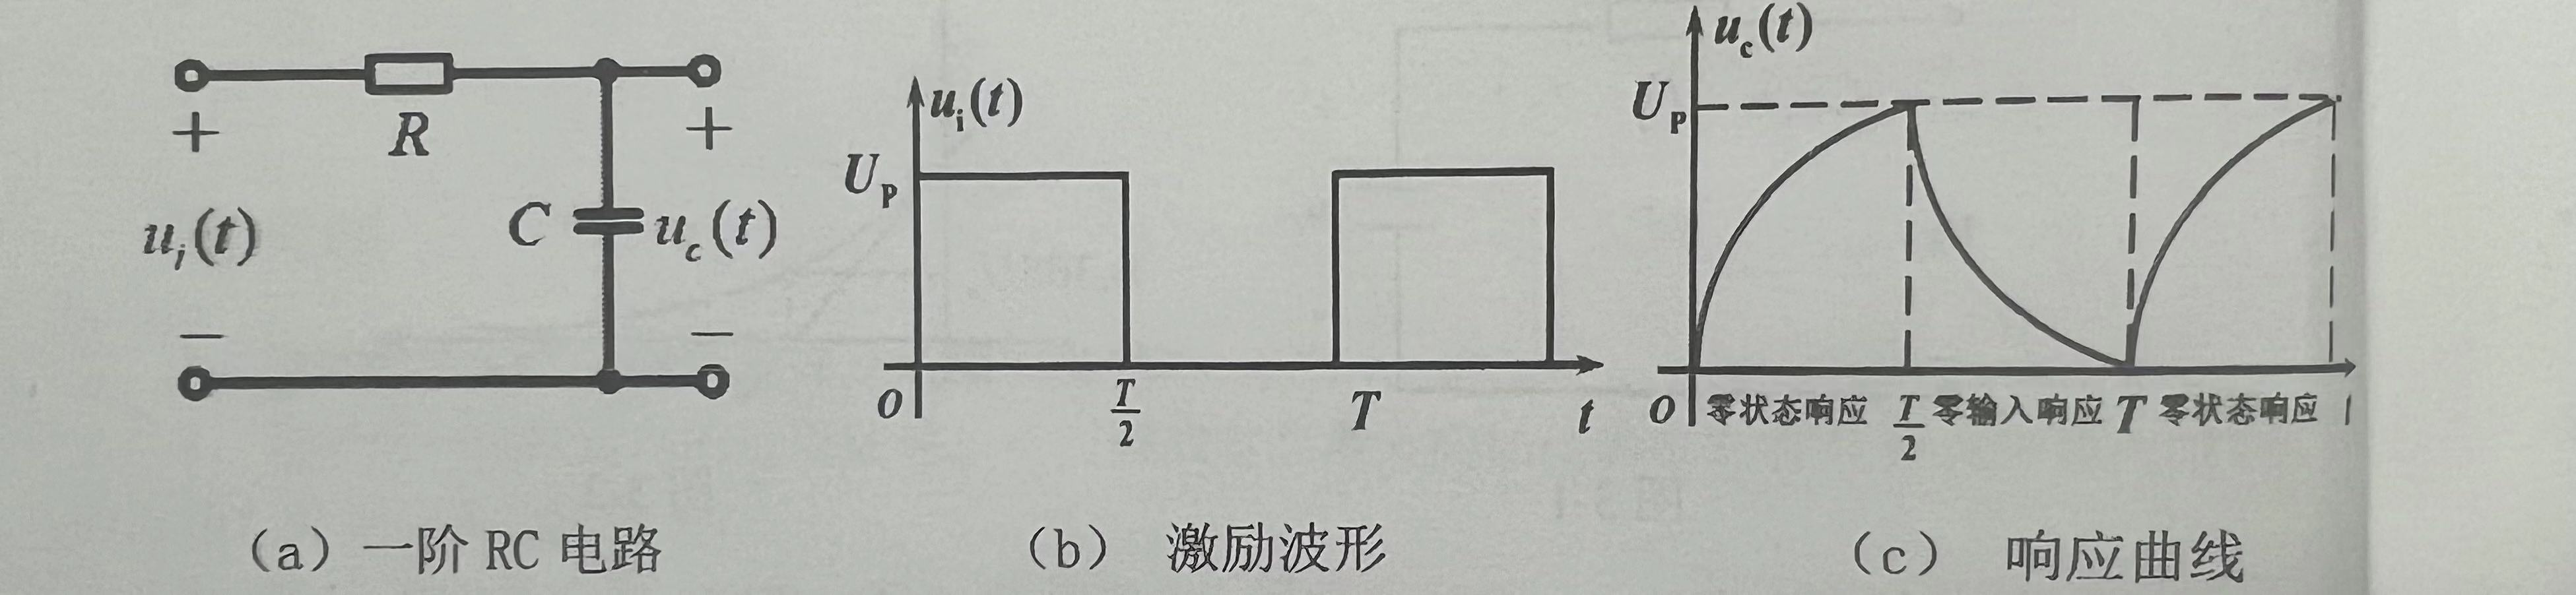
\includegraphics[scale=0.08]{1}\\
        {\small 图一}
    \end{center}

    {{零状态响应:电路中的储能原件原始储能为零,仅由独立电源作用引起的响应。输入阶跃电压$u_{i}(t) = U_{p}u(t)$,由电路中微分方程}}

    \begin{equation}
        \left\{
        \begin{array}{c}
            RC\frac{d U_{c}(t)}{d t}=U_{P} \\
            u_{c}(0^{+})=0
        \end{array}
        \right.\label{eq:equation}
    \end{equation}

    {{得零状态响应$u_{c}(t) = U_{P}\left(1 − e^{-\frac{t}{RC}}\right)$, 即输出电压$u_{c}(t)$按指数规律由 0 趋于$U_{P}$, 其中响应时间常数$\tau =RC$,此时$u_{c}(t)=0.632U_{P}$。}}

    {{零输入响应:换路后无独立电源的电路中,仅由储能元件原始储能引起的的响应。 以电容为例,电容的原始储能为$u_{c}(t_{p}) = U_{P}$,由电路中微分方程}}

    \begin{equation}
        \left\{
        \begin{array}{c}
        (R_{1}+R)
            C\frac{d U_{c}(t)}{d (t)}+u_{c}=0 \\
            u_{c}(\frac{T}{2})=U_{P}
        \end{array}
        \right.\label{eq:equation2}
    \end{equation}

    {{得零状态响应$u_{c}(t) = U_{P} e^{-\frac{t}{(R_{1}+R)C}})$, 即输出电压$u_{c}(t)$按指数规律由 0 趋于$U_{P}$, 其中响应时间常数$\tau =(R_{1}+R)C$,此时$u_{c}(t)=0.368U_{P}$。}}

    \subsection{一阶$RC$电路微分电路}\label{subsec:$rc$2}
    \begin{center}
        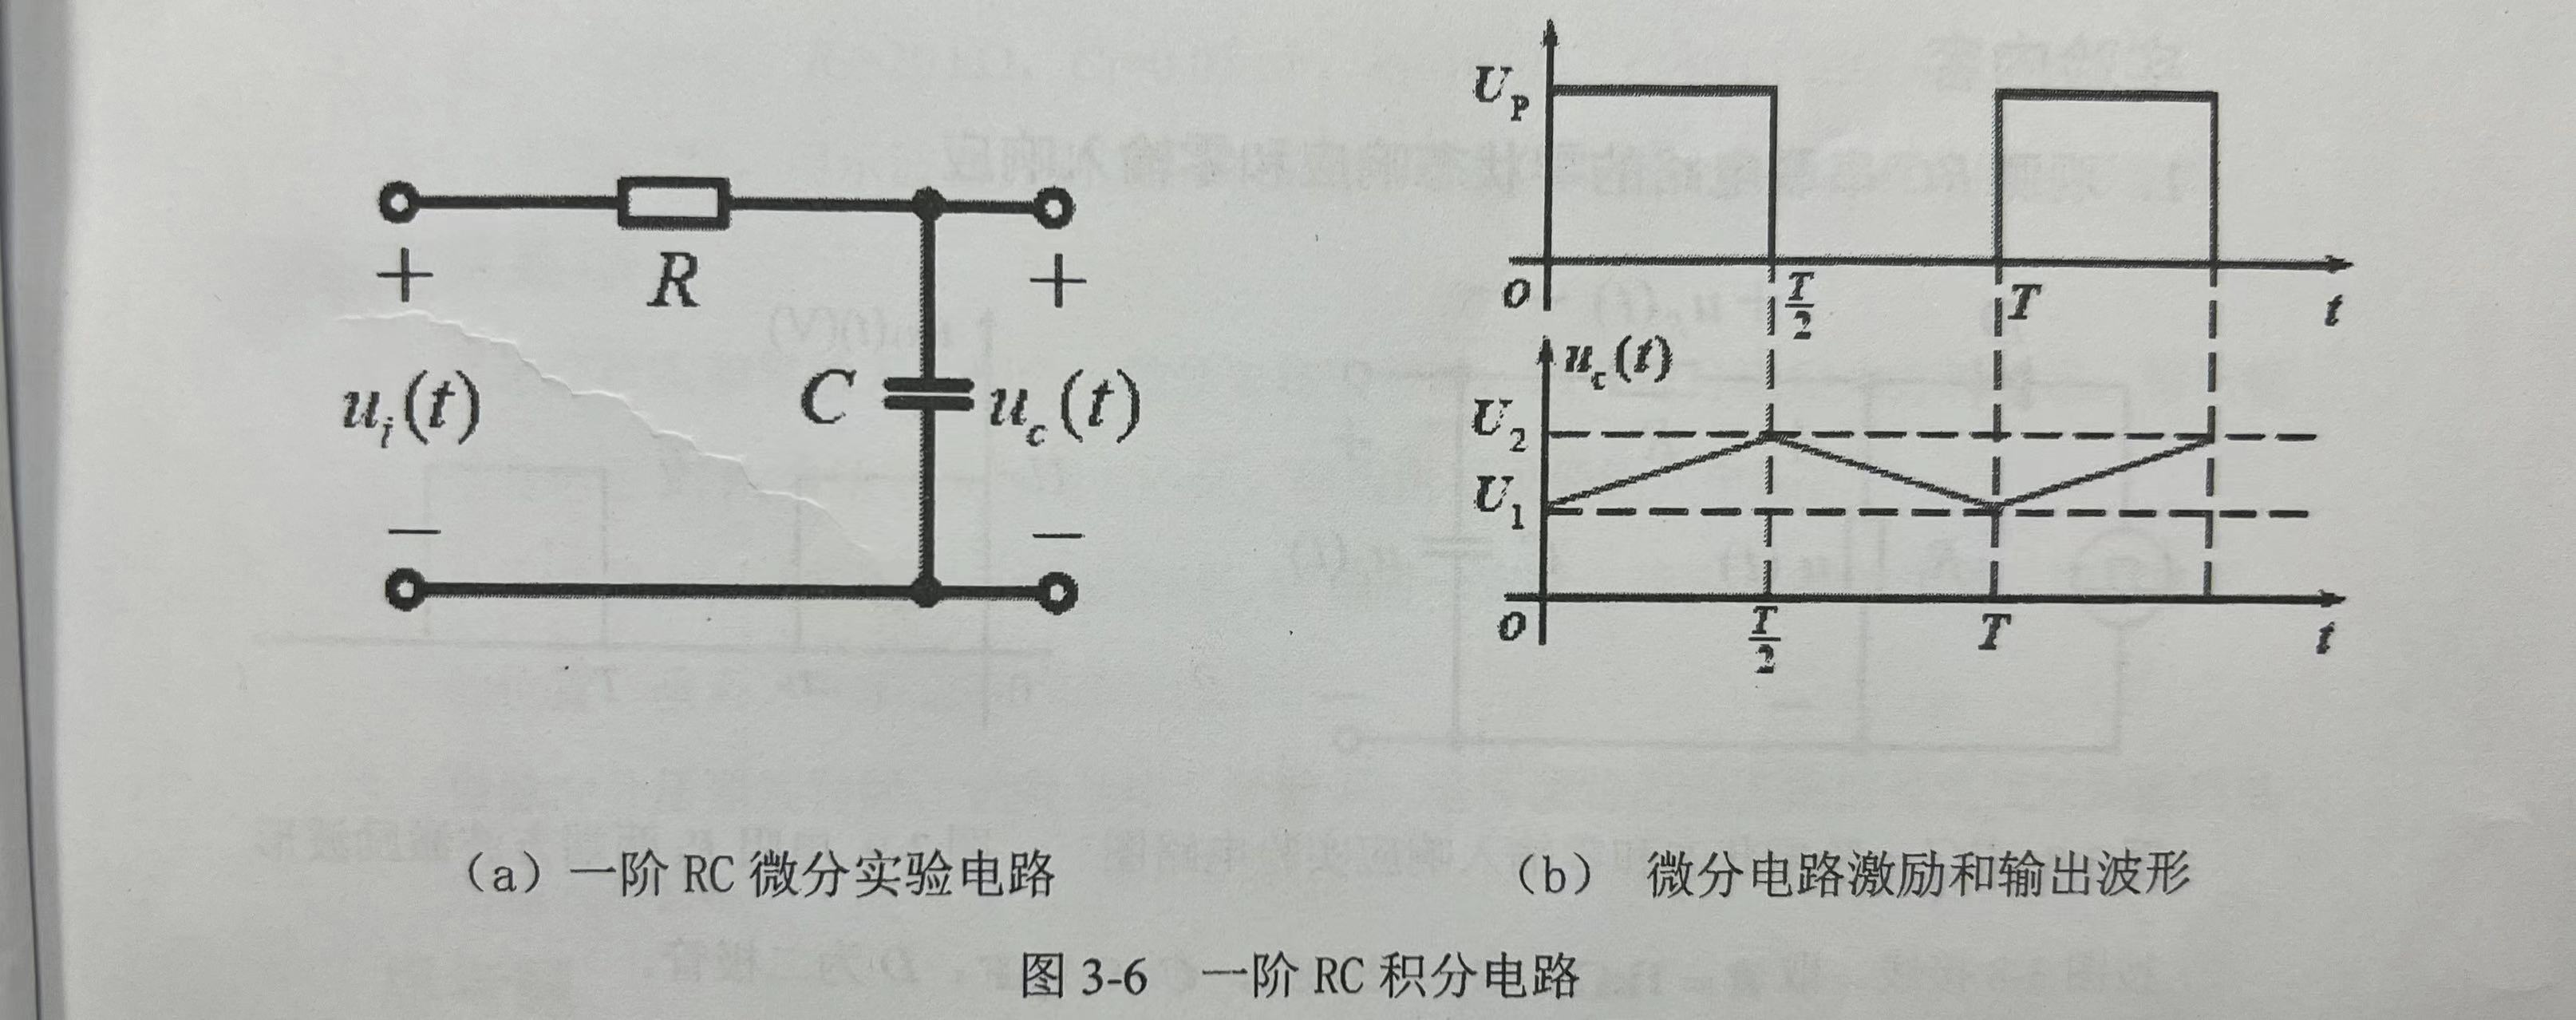
\includegraphics[scale=0.09]{2}\\
        {\small 图三}
    \end{center}

    {{当$t_{p}\gg\tau$ 有}}

    \begin{equation}
        \left\{
        \begin{array}{c}
            u_{R}(t)=Ri_{c} \approx \tau \frac{d P_(t)}{d t} \\
            u_{c}(t)\approx P(t)
        \end{array}
        \right.\label{eq:equation3}
    \end{equation}

    {{即从电阻上输出电压$u_{R}(t)$为输入电压 $P(t)$的微分形式乘以时间常数$\tau$。}}

    \subsection{一阶$RC$电路积分电路}\label{subsec:$rc$3}
    \begin{center}
        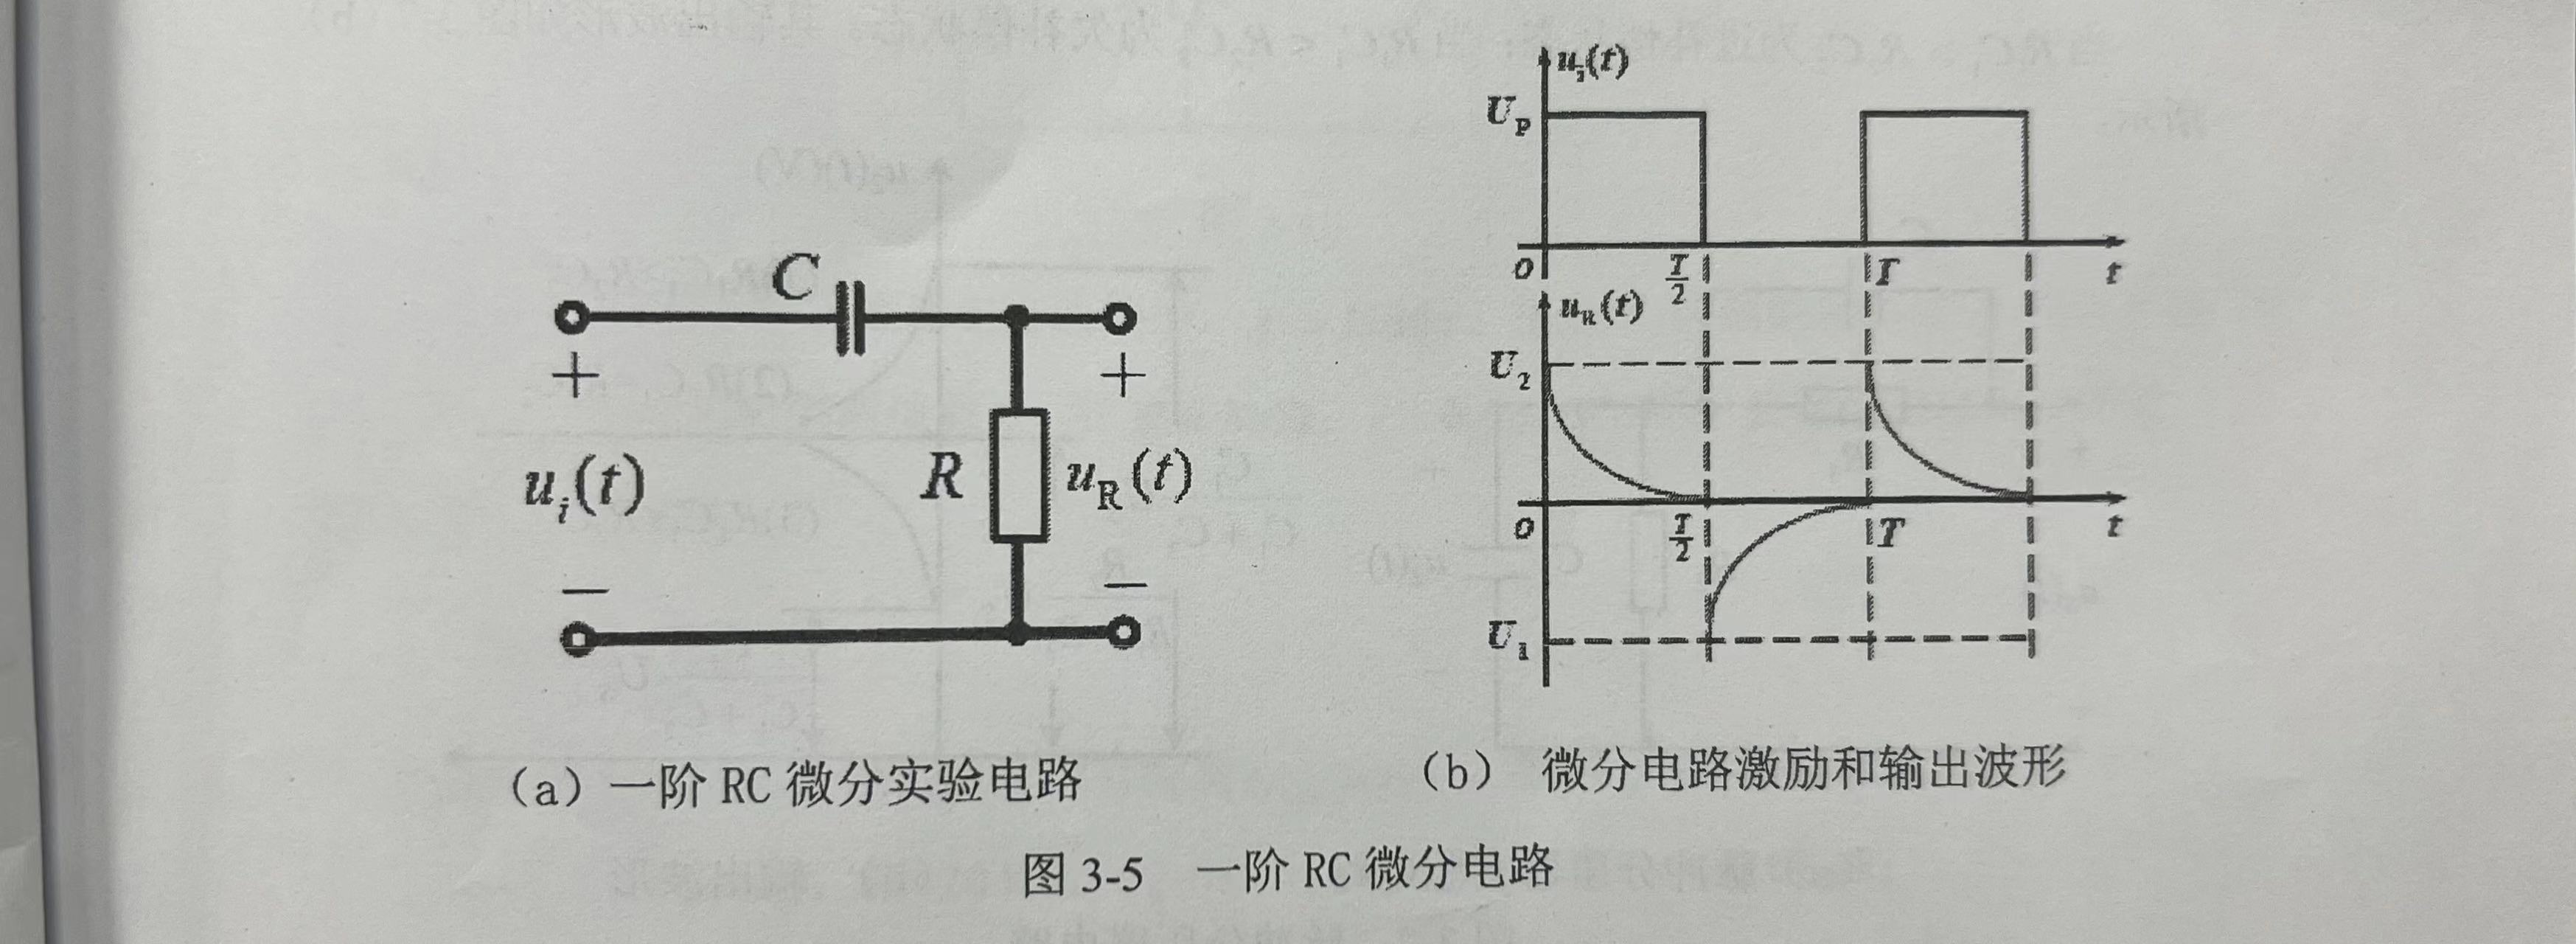
\includegraphics[scale=0.09]{3}\\
        {\small 图二}
    \end{center}

    {{当$t_{p}\ll\tau$ 有}}

    \begin{equation}
        \left\{
        \begin{array}{c}
            u_{c}(t)=\frac{1}{C} \int_{0}^{t} i_{c} d t \approx \frac{1}{\tau} \int_{0}^{t} P(t) d t\\
            u_{c}(t)\approx P(t)
        \end{array}
        \right.\label{eq:equation4}
    \end{equation}

    {{即从电阻上输出电压$u_{R}(t)$为输入电压 $P(t)$的微分形式乘以时间常数$\tau$。}}

    \vspace{1cm}


    \section{实验内容与方法}\label{sec:3}

    \subsection{一阶$RC$电路零输入响应和零状态响应}
    {测量一阶 $RC$ 电路零输入和零状态响应曲线以及时间常数$\tau$,其中 $U_{ip}=5V$,$f=500Hz$,$R_{1} =
    200\omega$, $R = 1k\omega$,$C = 0.1\mu F$,实验电路图如下图所示。}\label{subsec:$rc$4}

    \begin{center}
        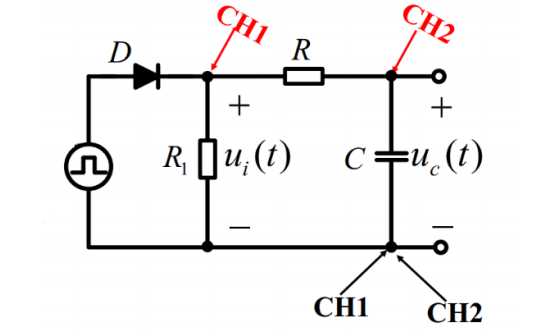
\includegraphics[scale=0.8]{4}\\
        {\small 图四}
    \end{center}

    \subsection{一阶$RC$电路积分电路}
    {观察记录一阶 $RC$ 积分电路的波形并测出 $U_{1}$,$U_{2}$,其中$U_{ip} = 5V$, $f = 1kHz$,$R_{1} = 200\omega$, $C =
    1\mu F$,$ R = 5k\omega$, 实验电路图如下图所示。}\label{subsec:$rc$5}

    \begin{center}
        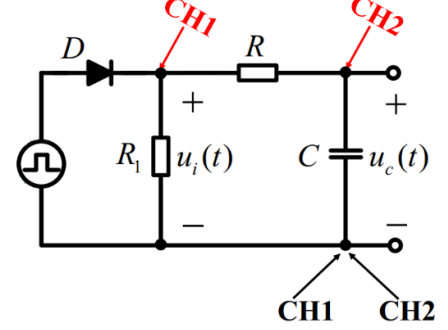
\includegraphics[scale=0.8]{5}\\
        {\small 图五}
    \end{center}

    \subsection{一阶$RC$电路微分电路}
    {观察记录一阶 $RC$ 微分电路的波形并测出 $U$ 值,其中$U_{ip} = 5V$, $f = 1kHz$,$R_{1} = 200\omega$, $C =
    0.05\mu F$,$R = 1k\omega$, 实验电路图如下图所示。}\label{subsec:$rc$6}

    \begin{center}
        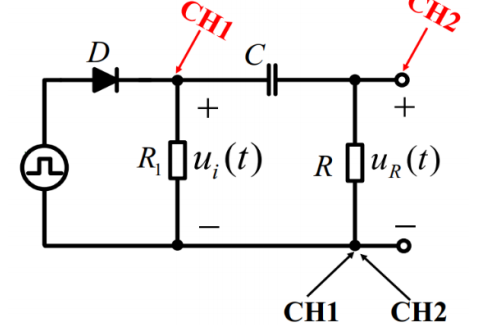
\includegraphics[scale=0.8]{6}\\
        {\small 图六}
    \end{center}

    \subsection{脉冲分压电路}
    {按照下图接线,输入方波信号幅度$U_{P-P}=6V$,频率$f=1KHz$。当$R_1=20K\Omega,C_1=0.005\mu F,R_2=10K\Omega,C_2=0.01\mu F$,此时电路正好补偿。}\label{subsec:}

    \begin{center}
        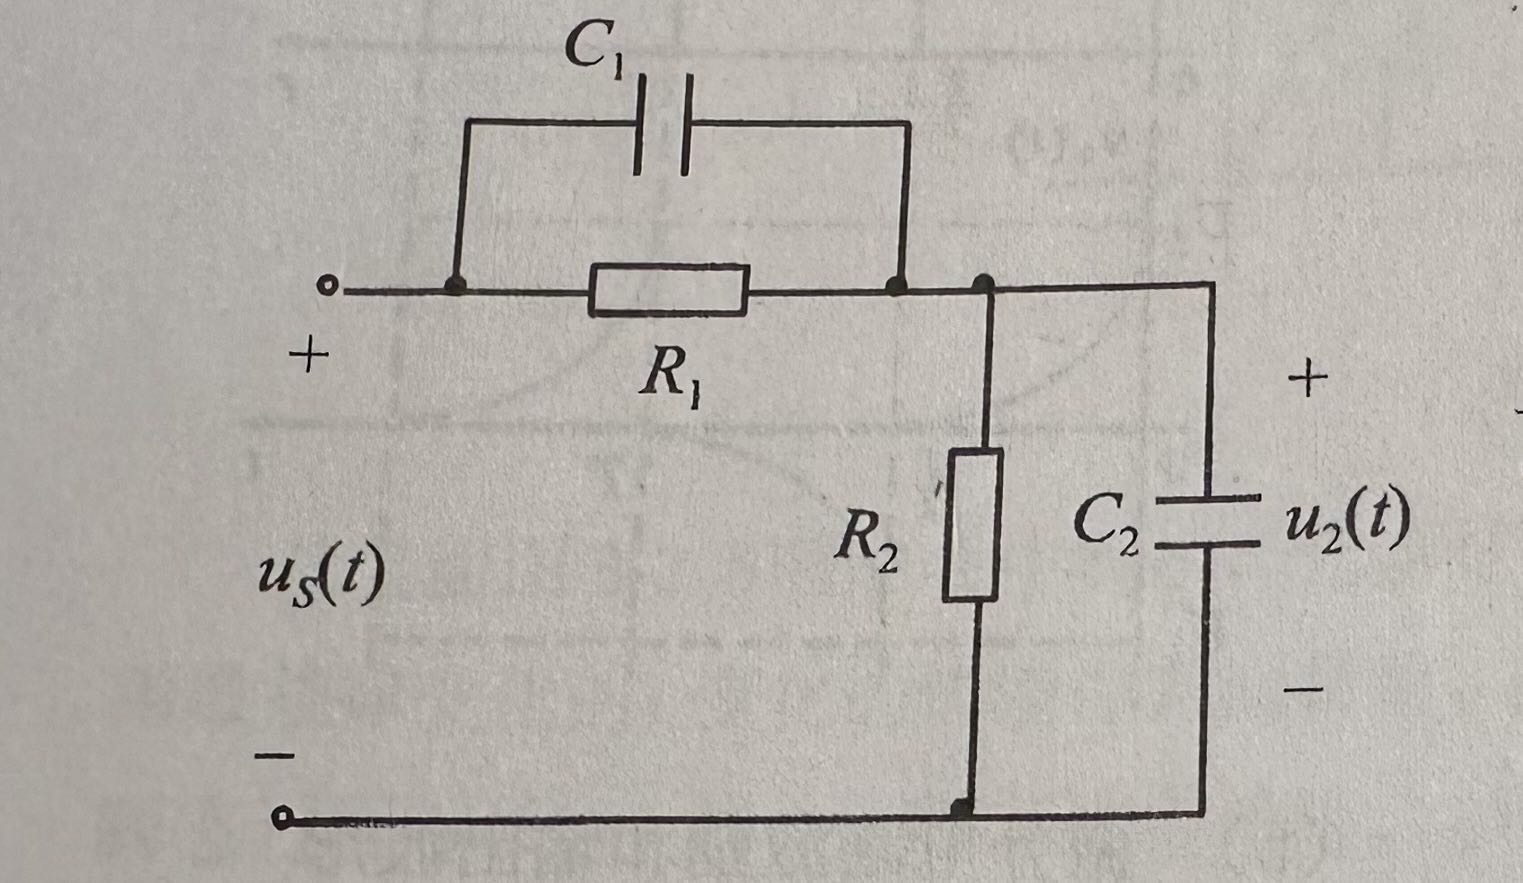
\includegraphics[scale=0.15]{15}\\
        {\small 图七}
    \end{center}

    \vspace{1cm}

    \section{实验仪器}
    {函数信号发生器,双踪示波器,万用表,二极管,电容箱,电阻箱,导线若干。}\label{sec:4}

    \vspace{1cm}


    \section{实验数据与误差分析}\label{sec:5}

    \subsection{一阶$RC$电路零输入响应和零状态响应}\label{subsec:$rc$7}
    \begin{figure*}[htb]
        \centering
        \subfloat[示波器图像]{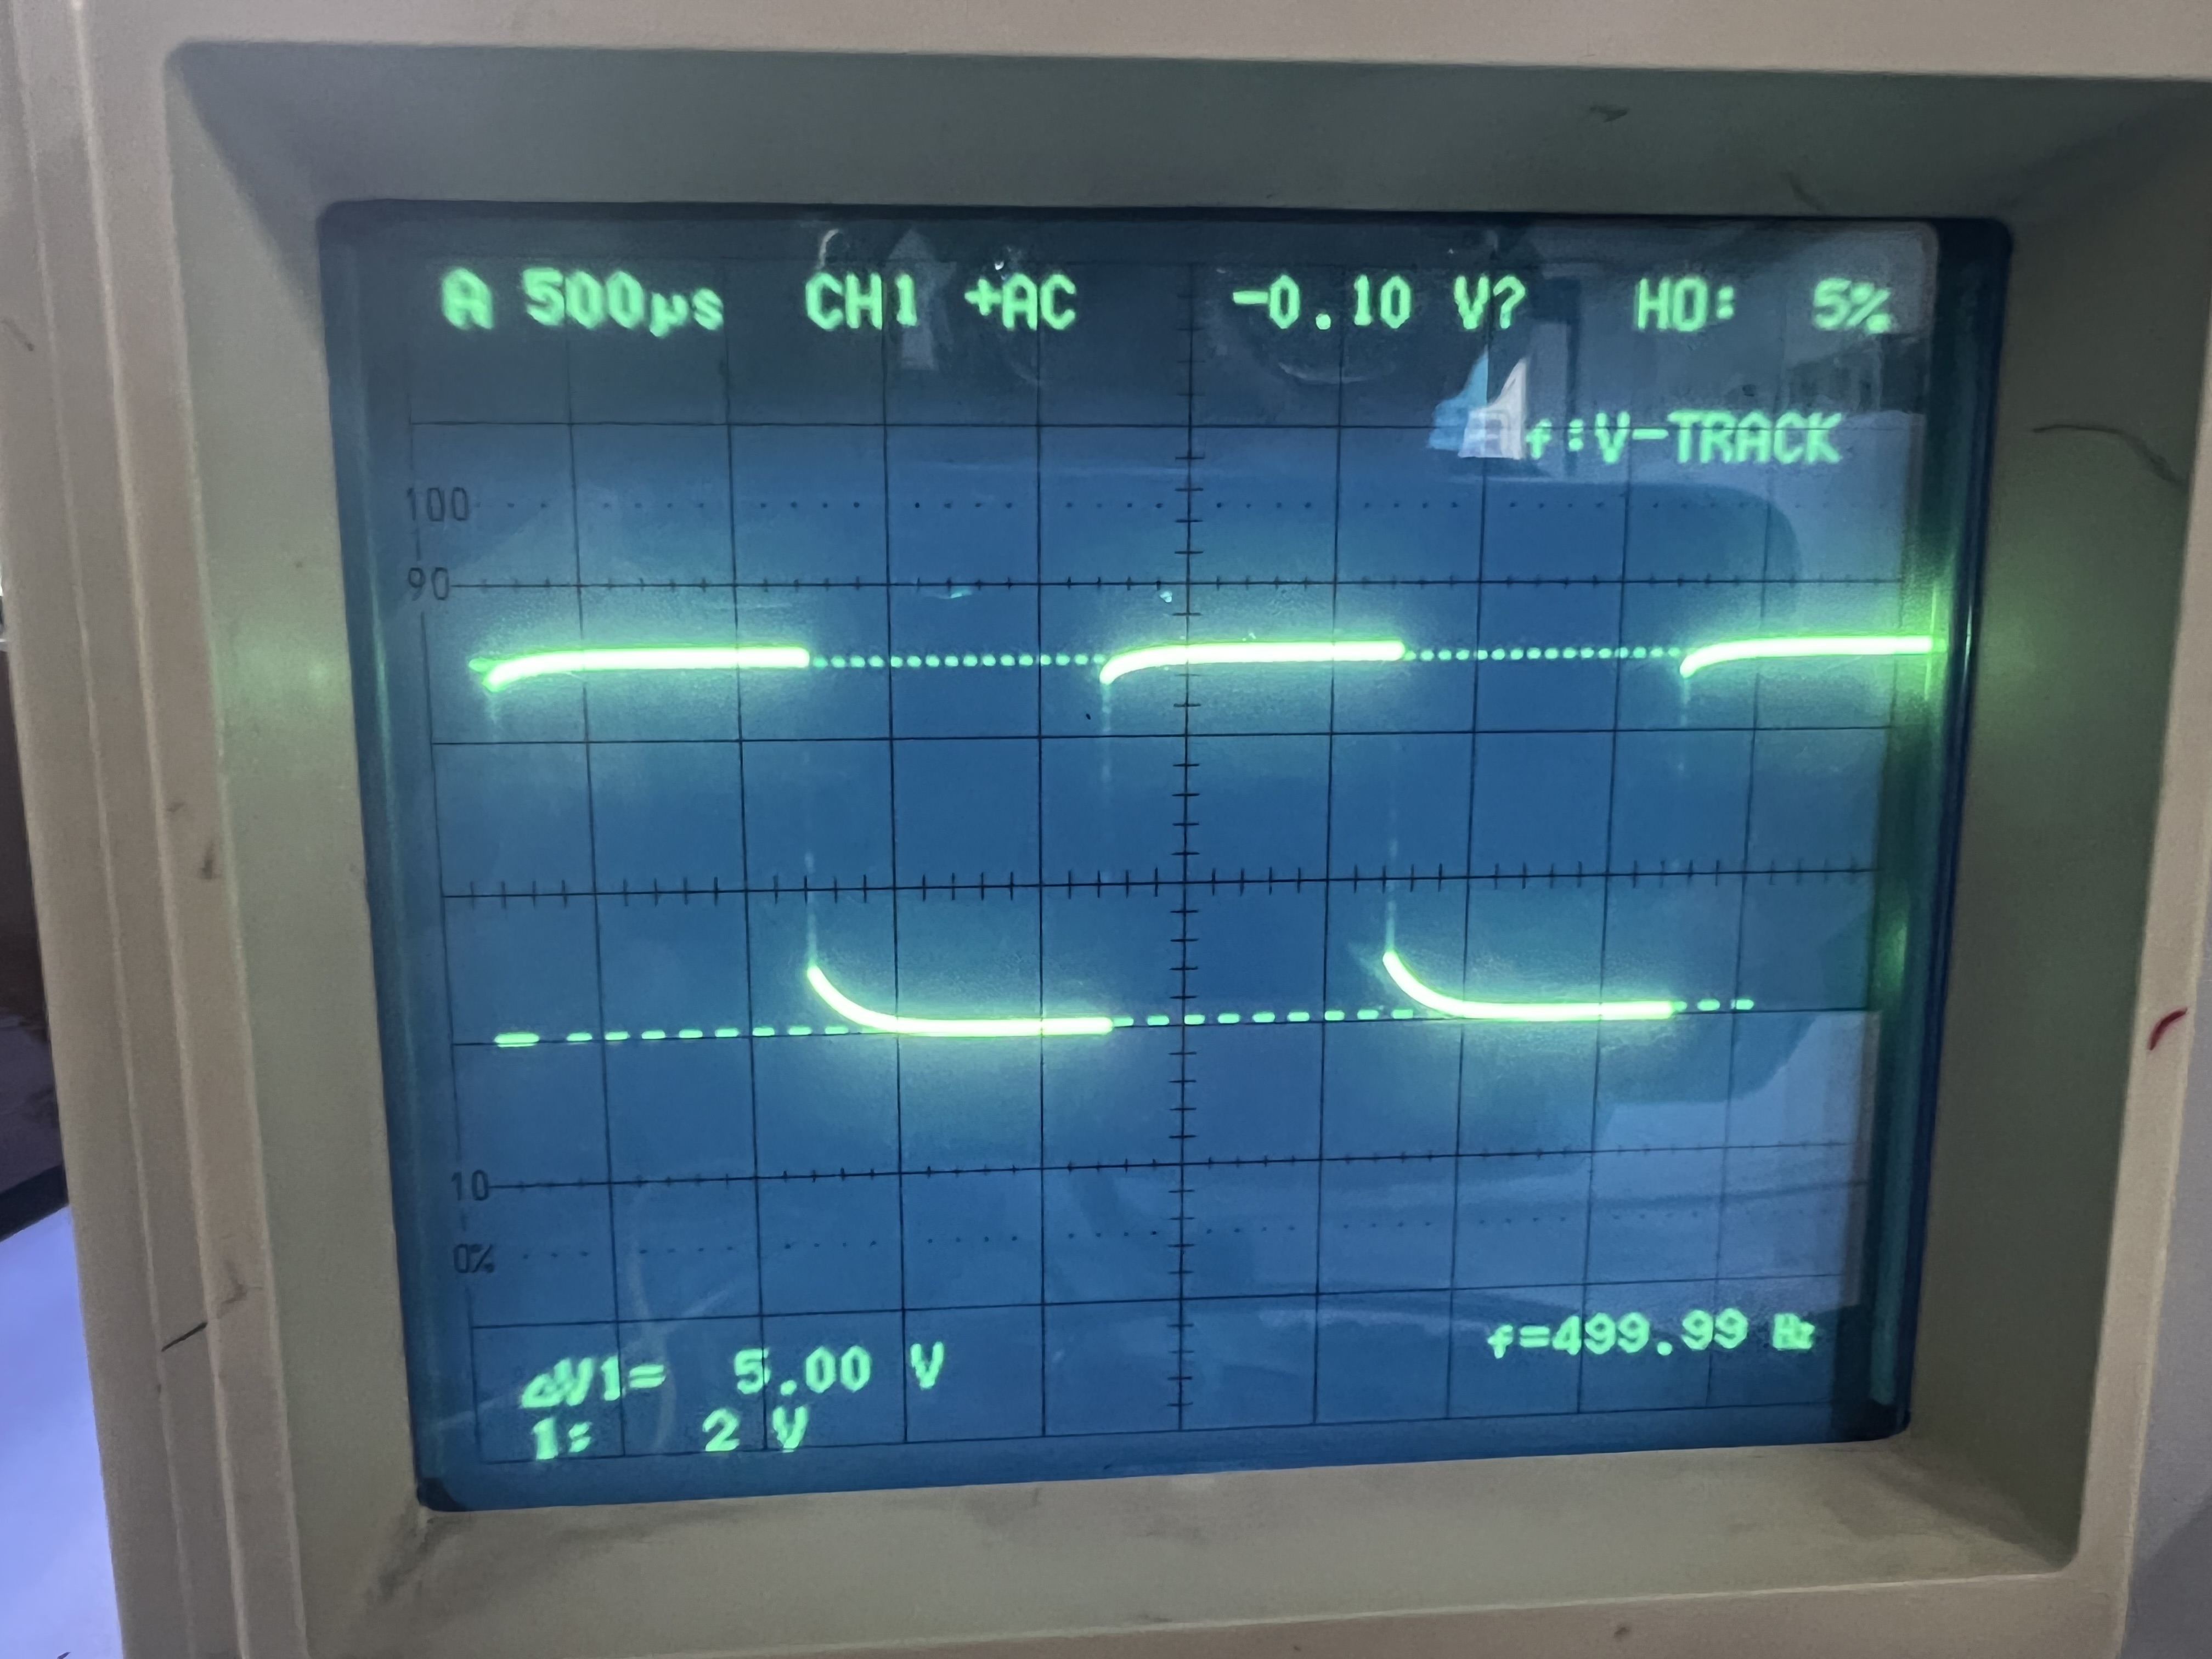
\includegraphics[scale=0.045]{7}}
        \subfloat[$u_c(t)$图像]{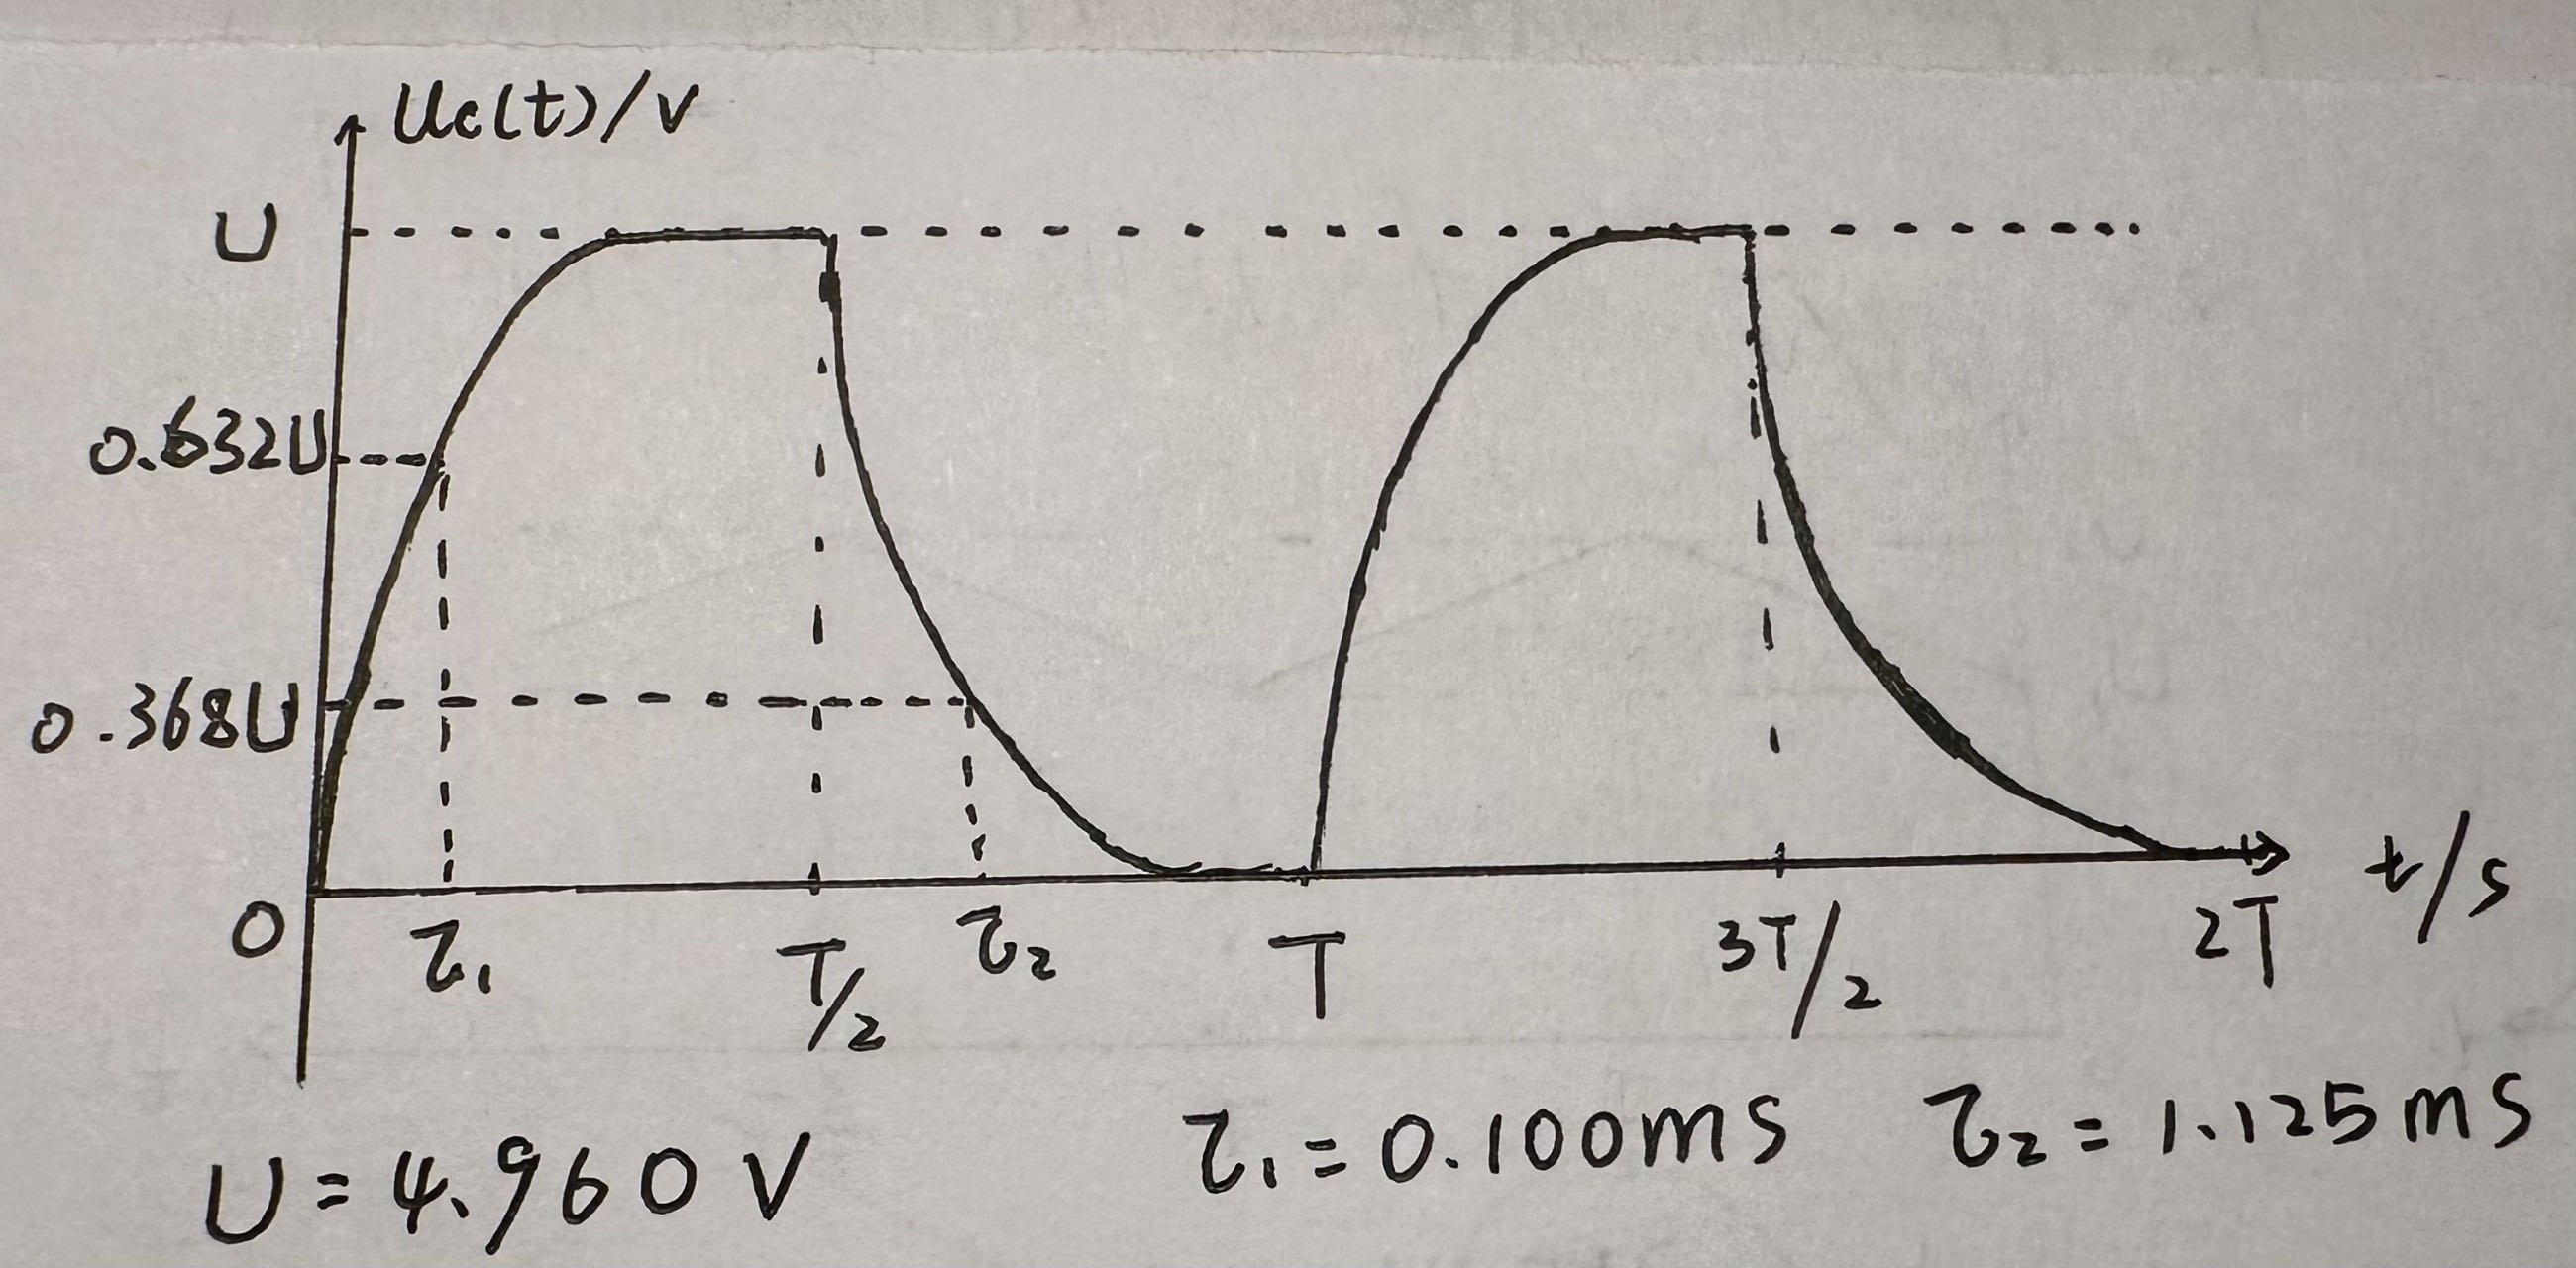
\includegraphics[scale=0.106]{8}}
        \caption{\small 图八:实验一相关图片}
    \end{figure*}

    {{由图八(a)分析可知,在$t_{P}\gg \tau$,$U_{R1}=5V$的情况下:电容$C$的阶跃响应为开端略有弯曲,后来近似峰值5V的方波;其零输入响应为开端略有弯曲,后来近似0V的方波。该结果与理论应该出现的方波大致吻合。 开端出现弯曲的原因是电容具有储存电荷,两端电压改变时可以短暂维持原状的能力。}}

    {{阶跃响应和零输入的波形参数如图八(b)所示,示波器图像见下图。}}

    \begin{figure*}[htb]
        \centering
        \subfloat[阶跃响应曲线]{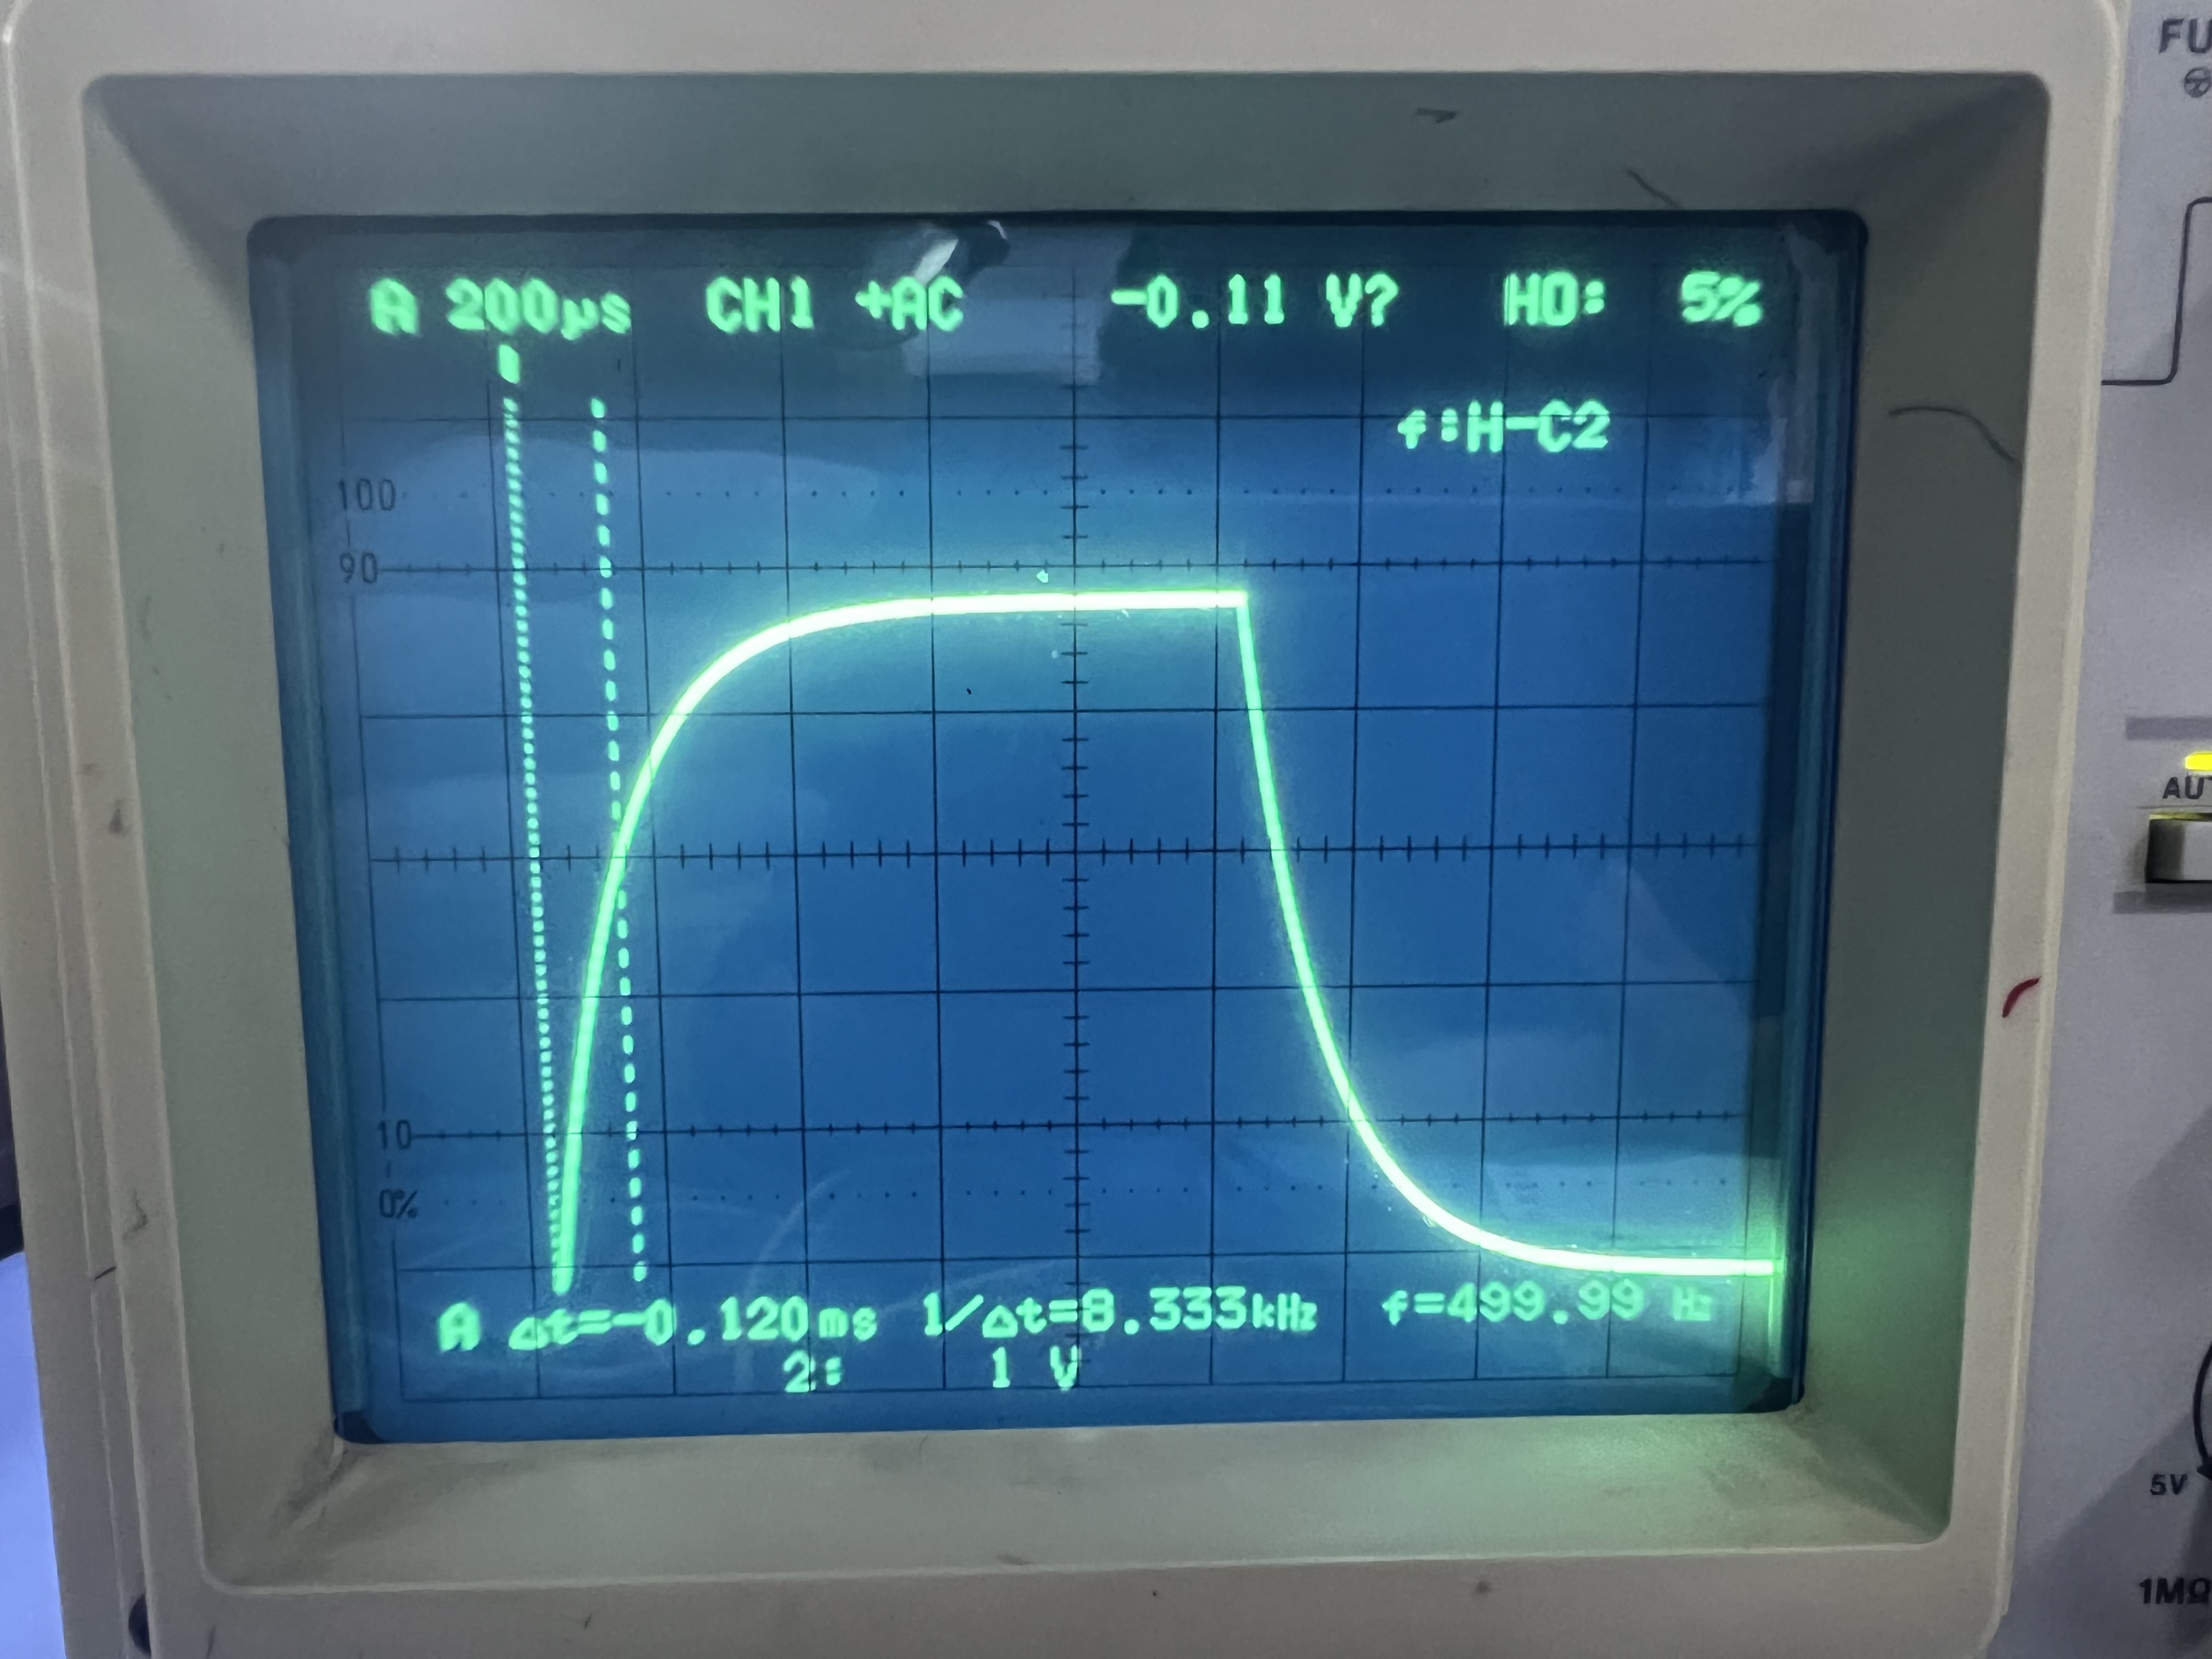
\includegraphics[scale=0.04]{9}}
        \subfloat[零输入响应曲线]{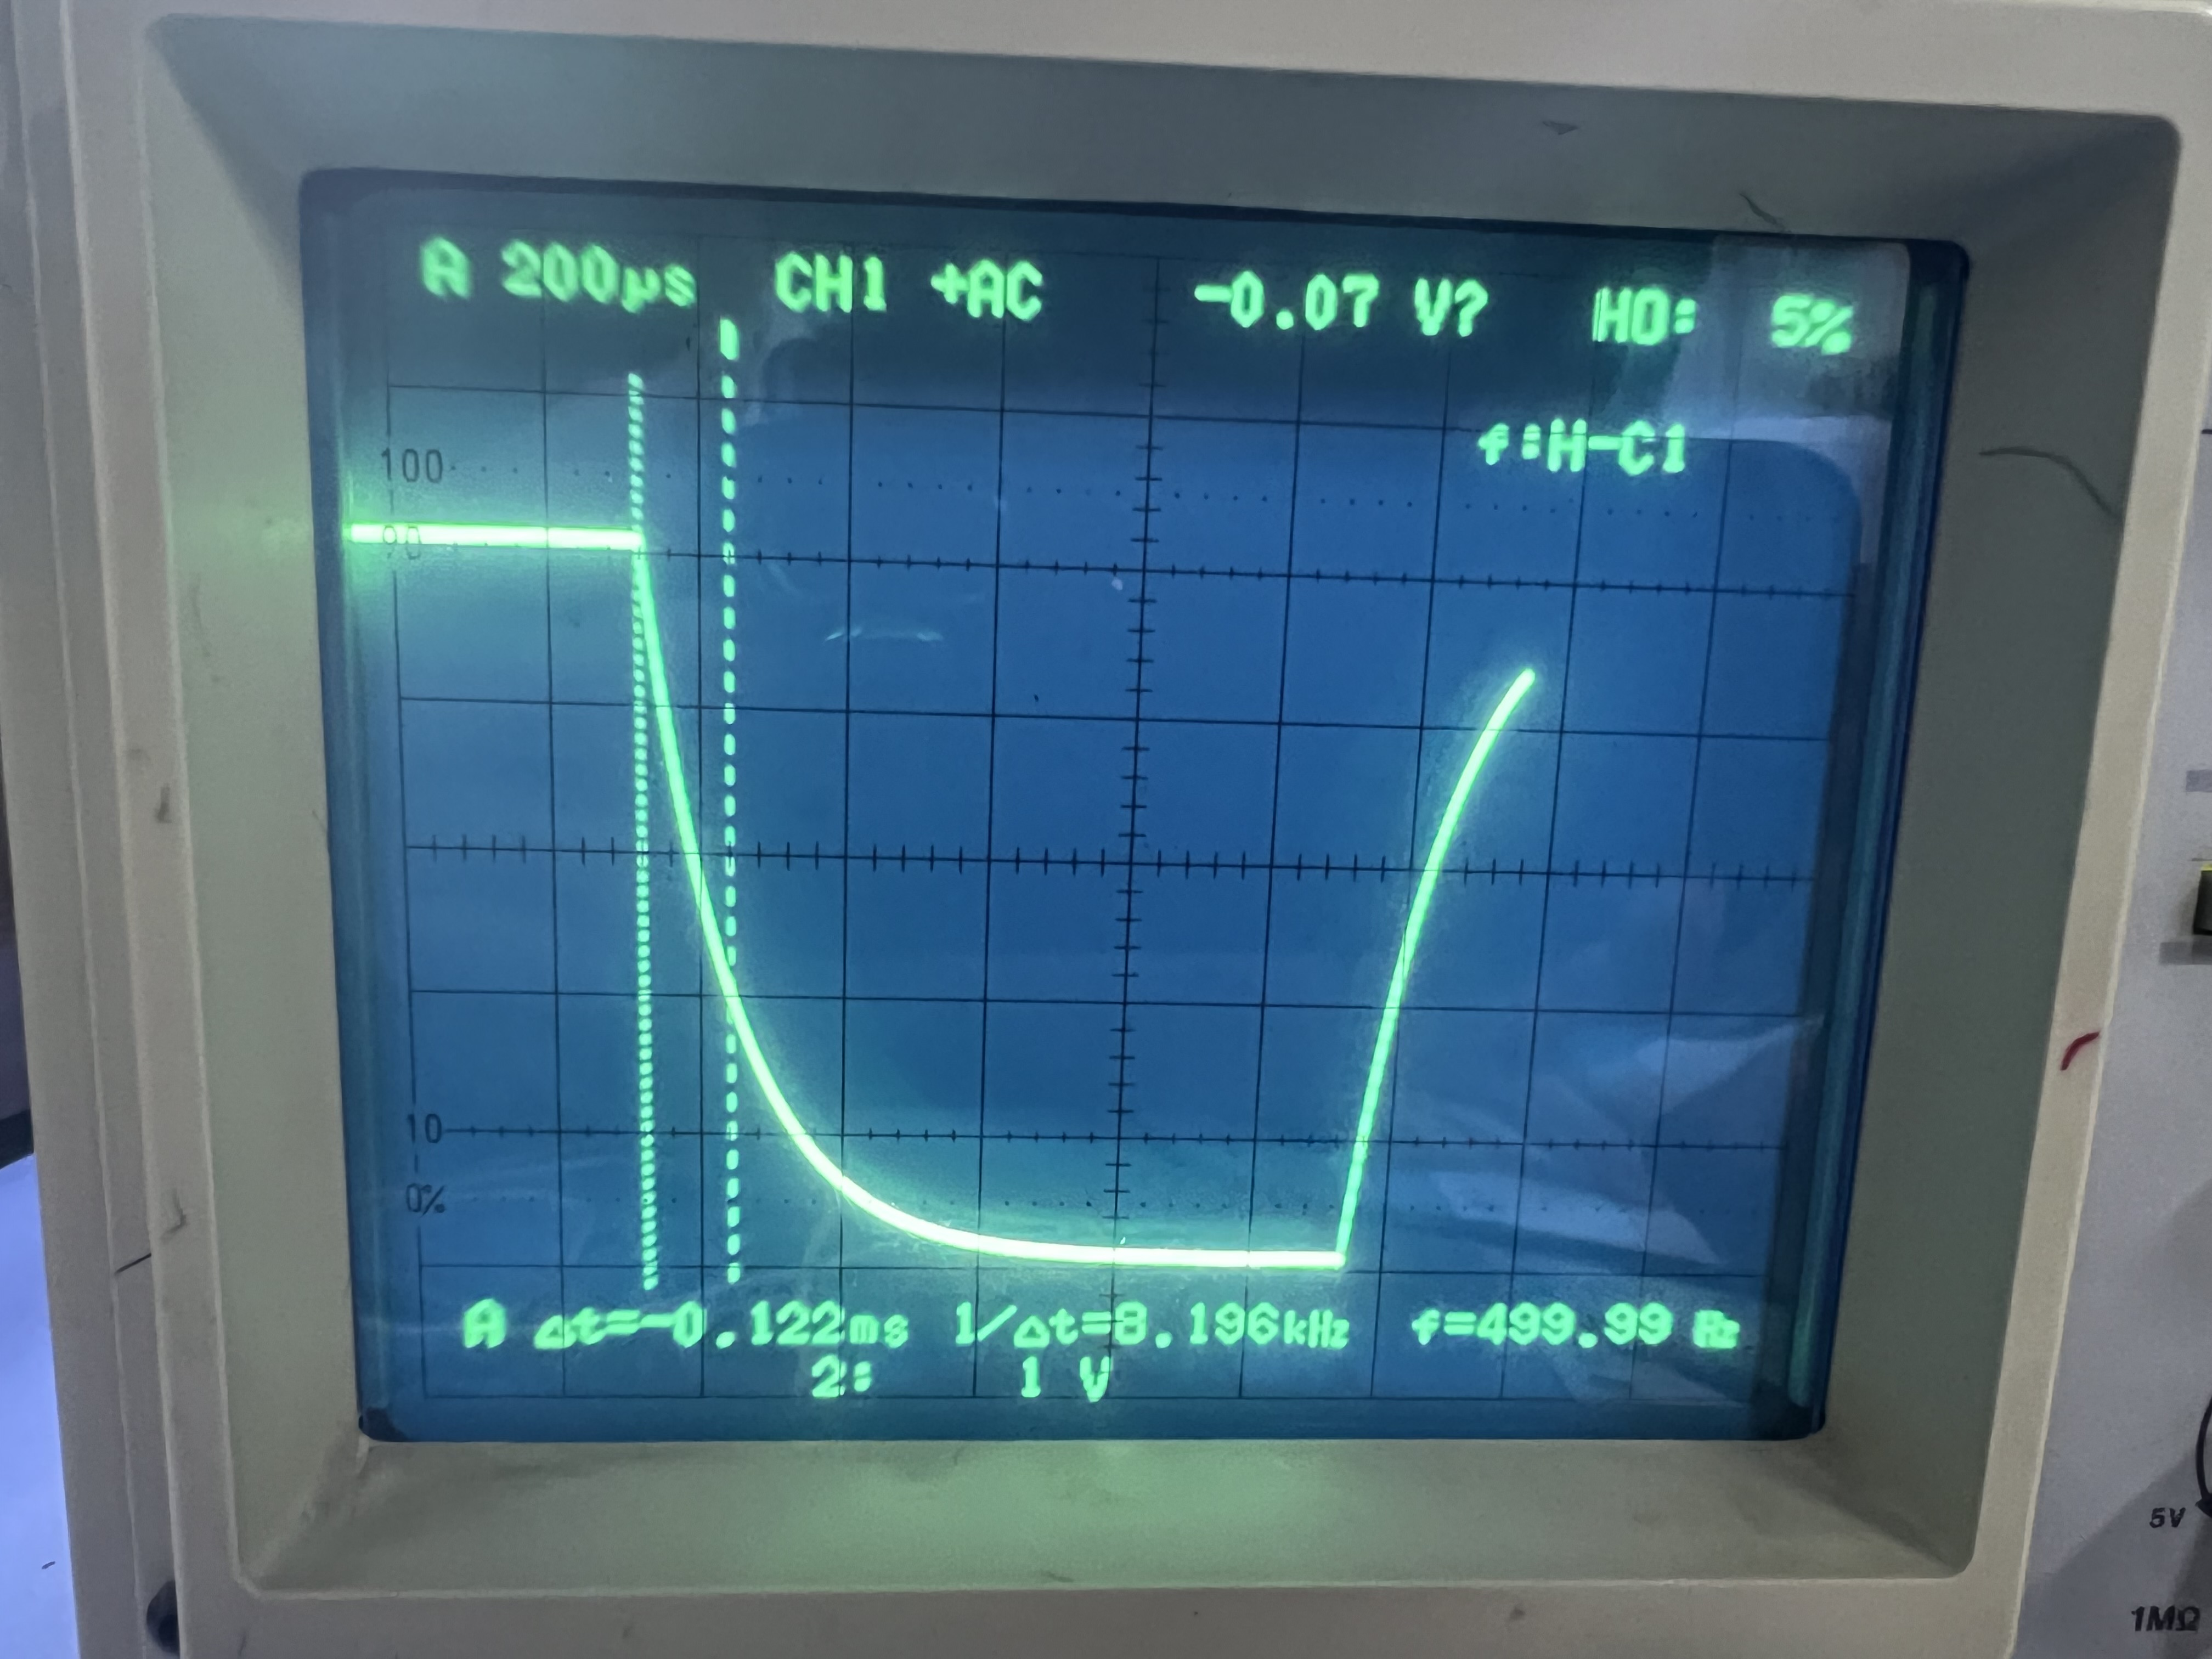
\includegraphics[scale=0.04]{10}}
        \caption{\small 图九:实验一相关图片}
    \end{figure*}

    \vspace{1cm}

    \subsection{一阶$RC$积分电路}\label{subsec:$rc$8}

    {{输出波形图像及波形参数如下图所示。}}

    \begin{figure*}[htb]
        \centering
        \subfloat{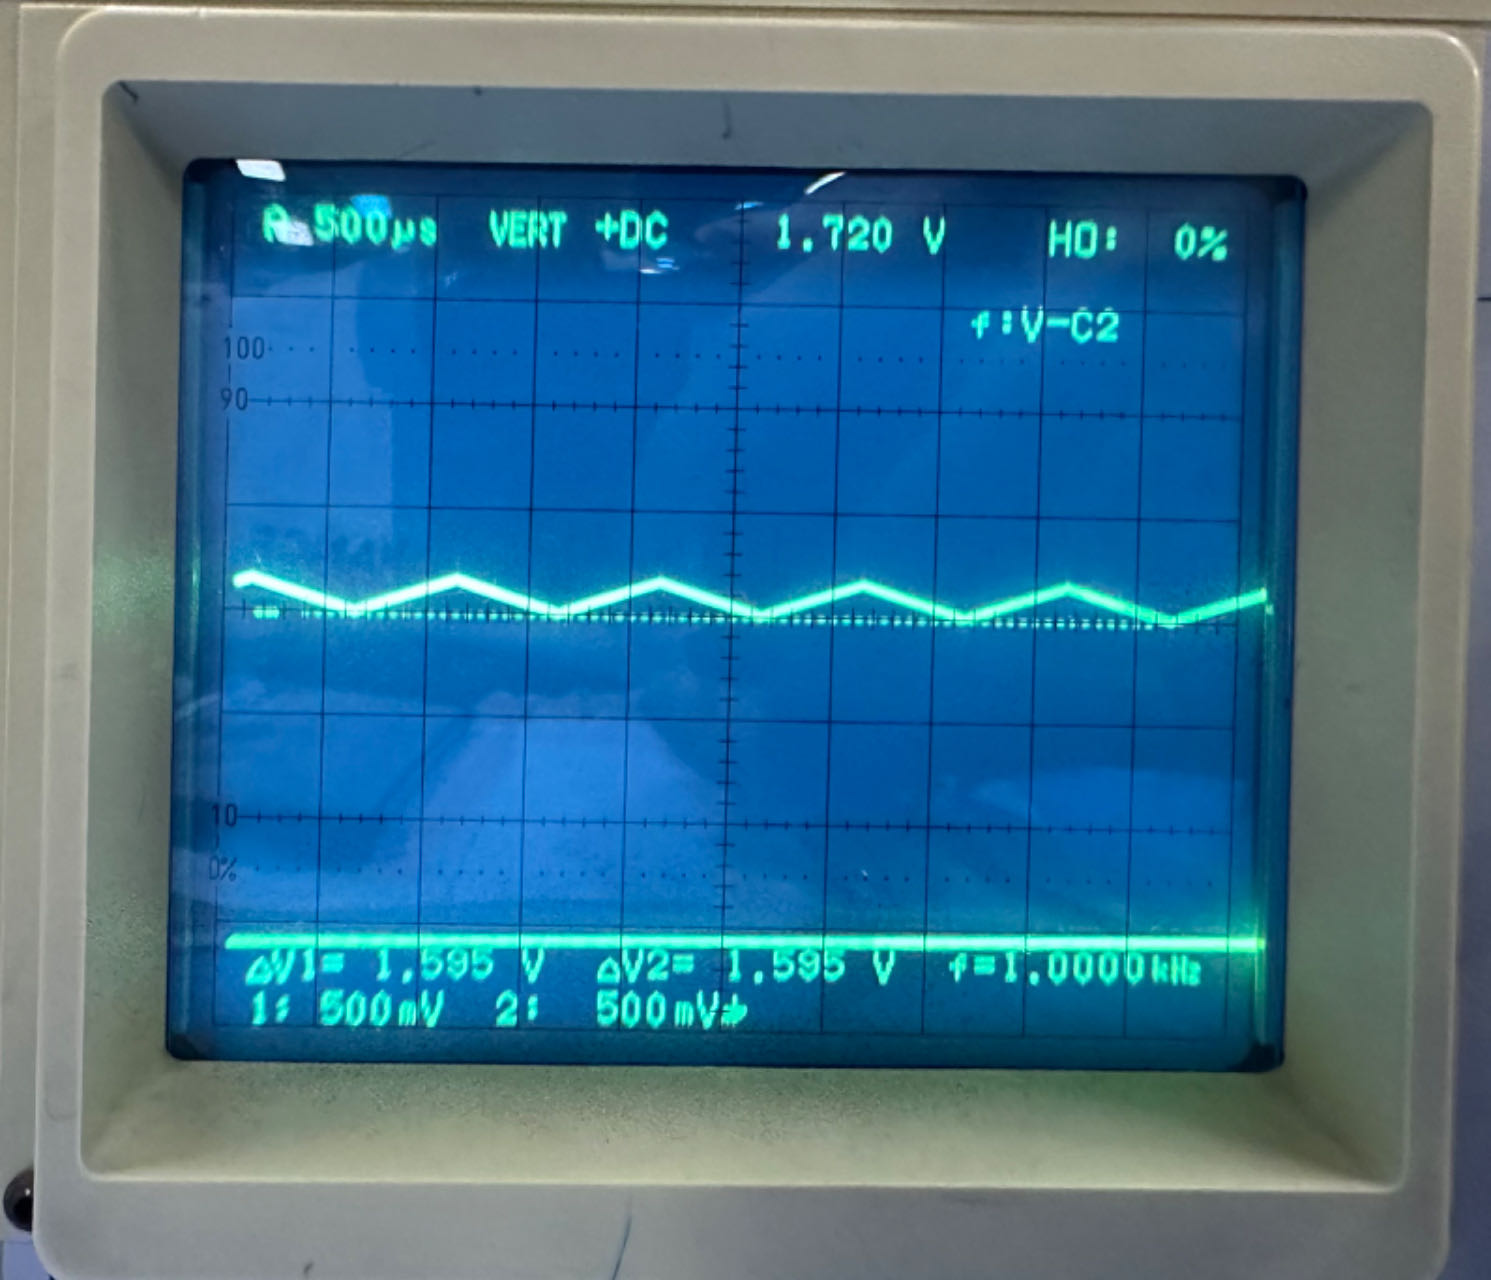
\includegraphics[scale=0.1]{13}}
        \subfloat{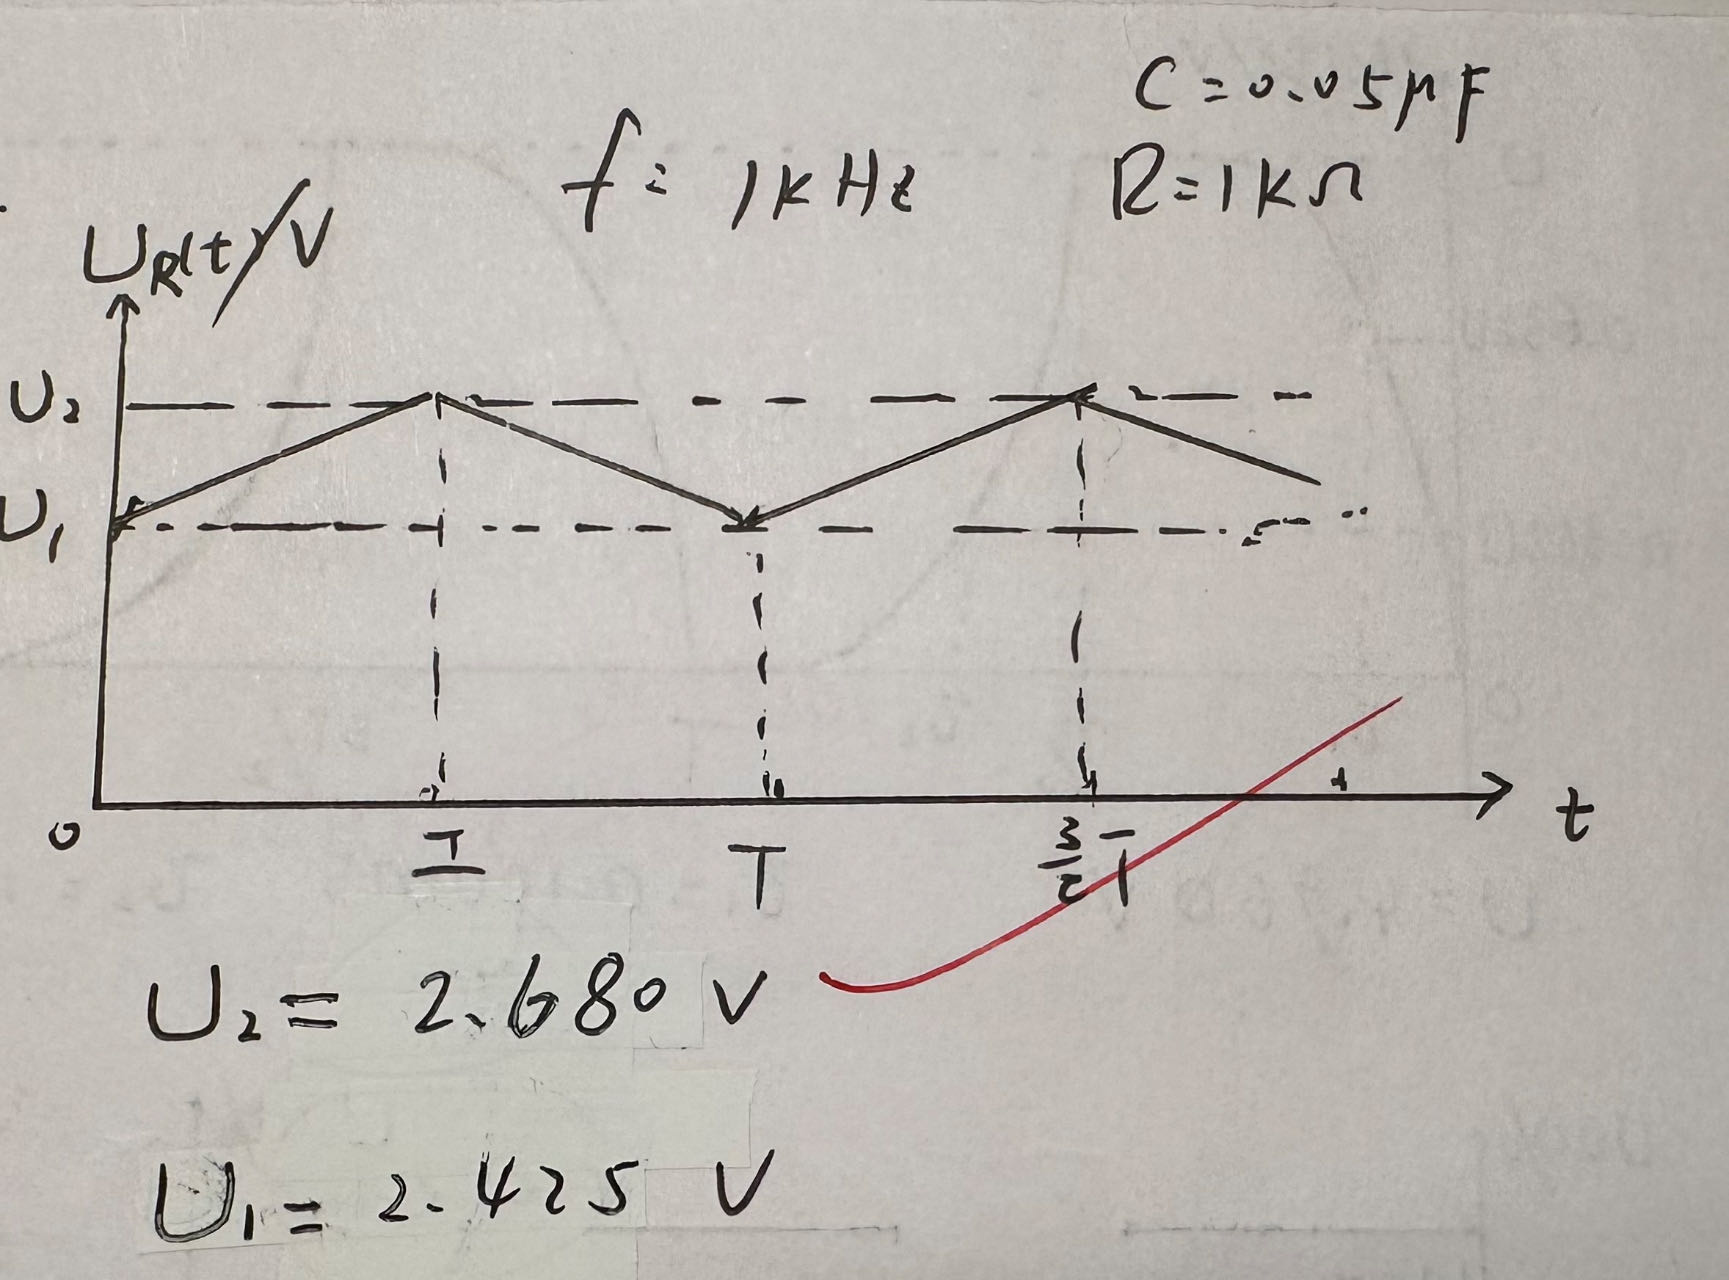
\includegraphics[scale=0.1]{14}}
        \caption{\small 图十:实验二相关图片}
    \end{figure*}

    \subsection{一阶$RC$微分电路}\label{subsec:$rc$9}

    {{输出波形图像及波形参数如下图所示。}}

    \begin{figure*}[htb]
        \centering
        \subfloat{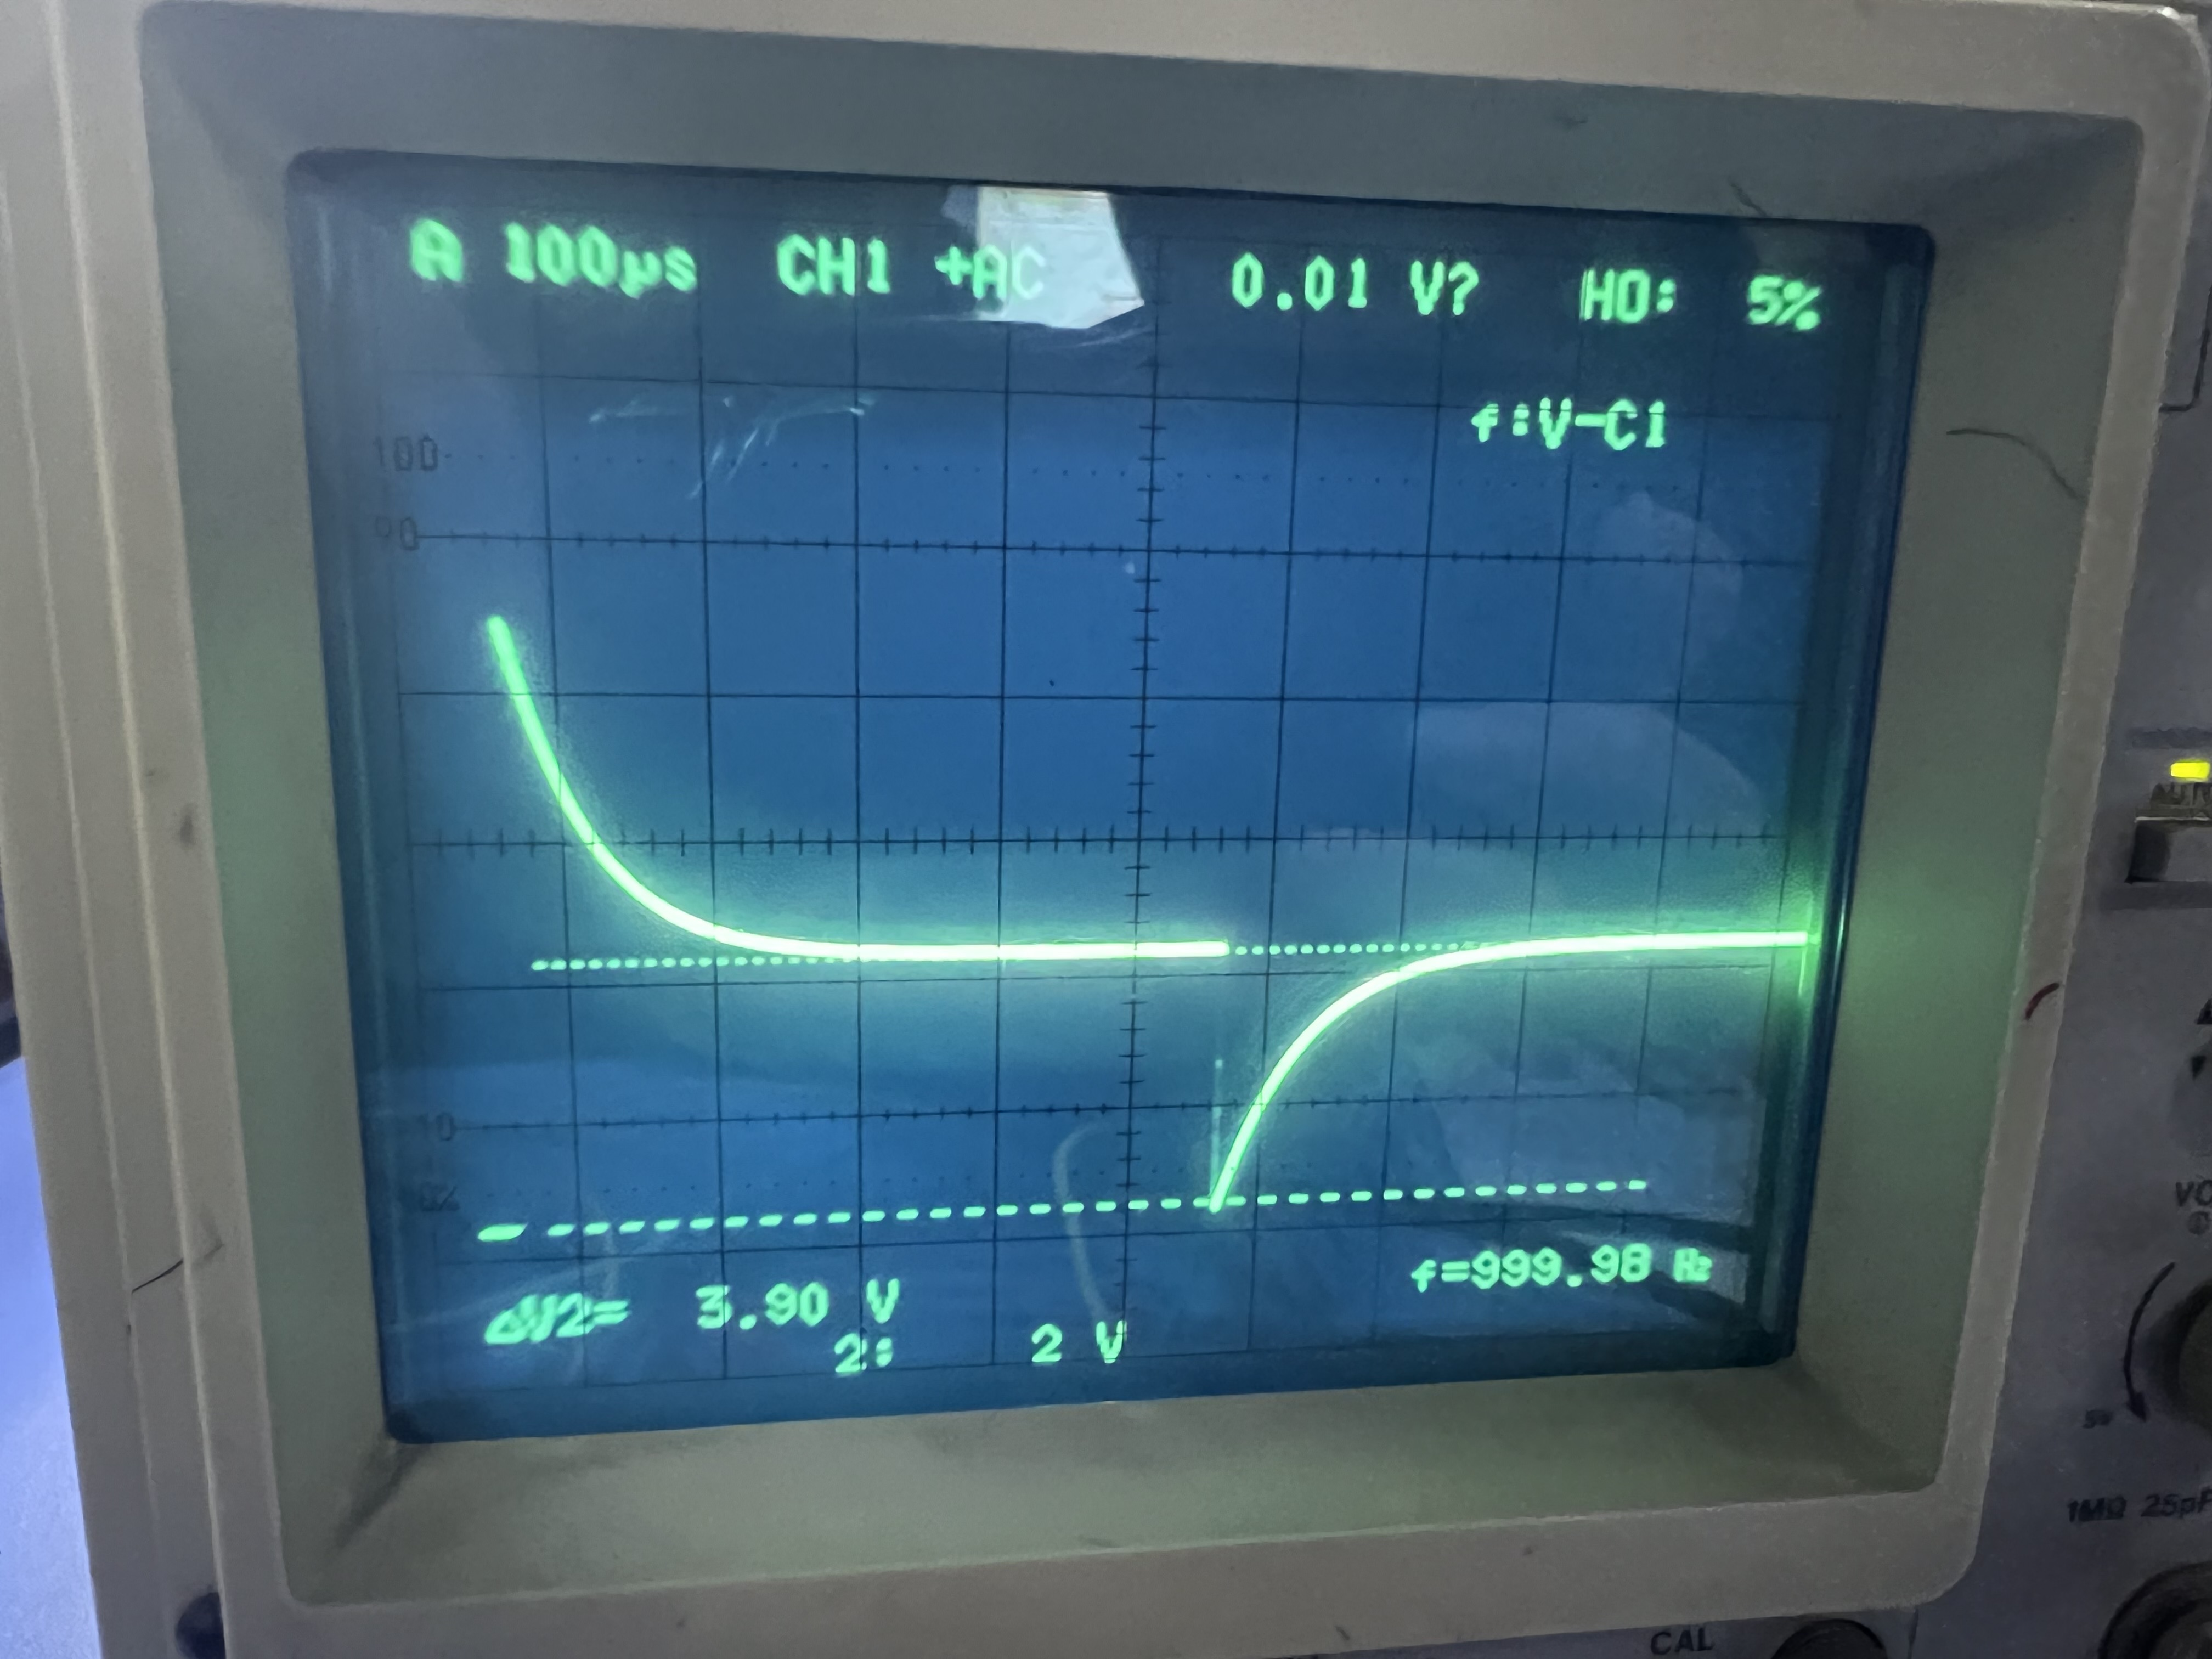
\includegraphics[scale=0.04]{11}}
        \subfloat{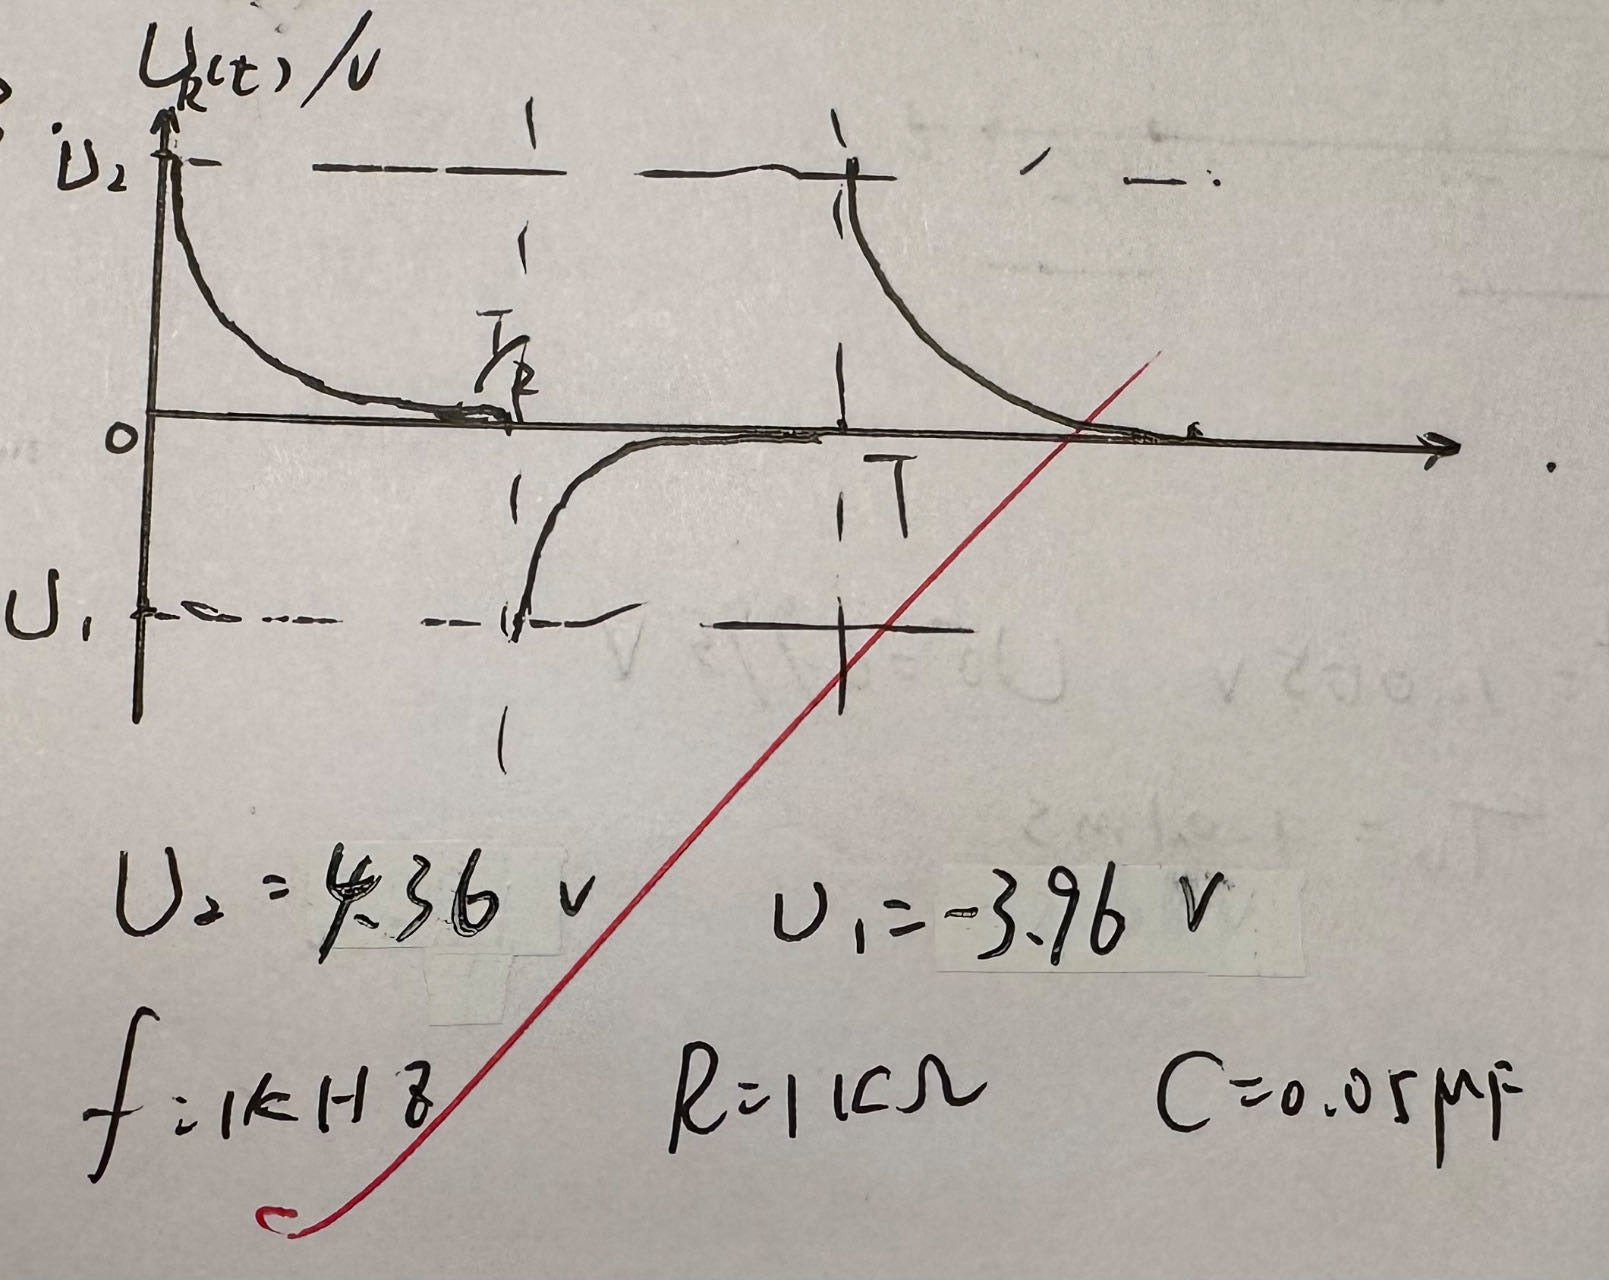
\includegraphics[scale=0.09]{12}}
        \centering
        \caption{\small 图十一:实验三相关图片}
    \end{figure*}

    \subsection{脉冲分压电路}\label{subsec:2}

    {{输出波形图像及波形参数如下图所示。}}

    \begin{figure*}[htb]
        \centering
        \subfloat{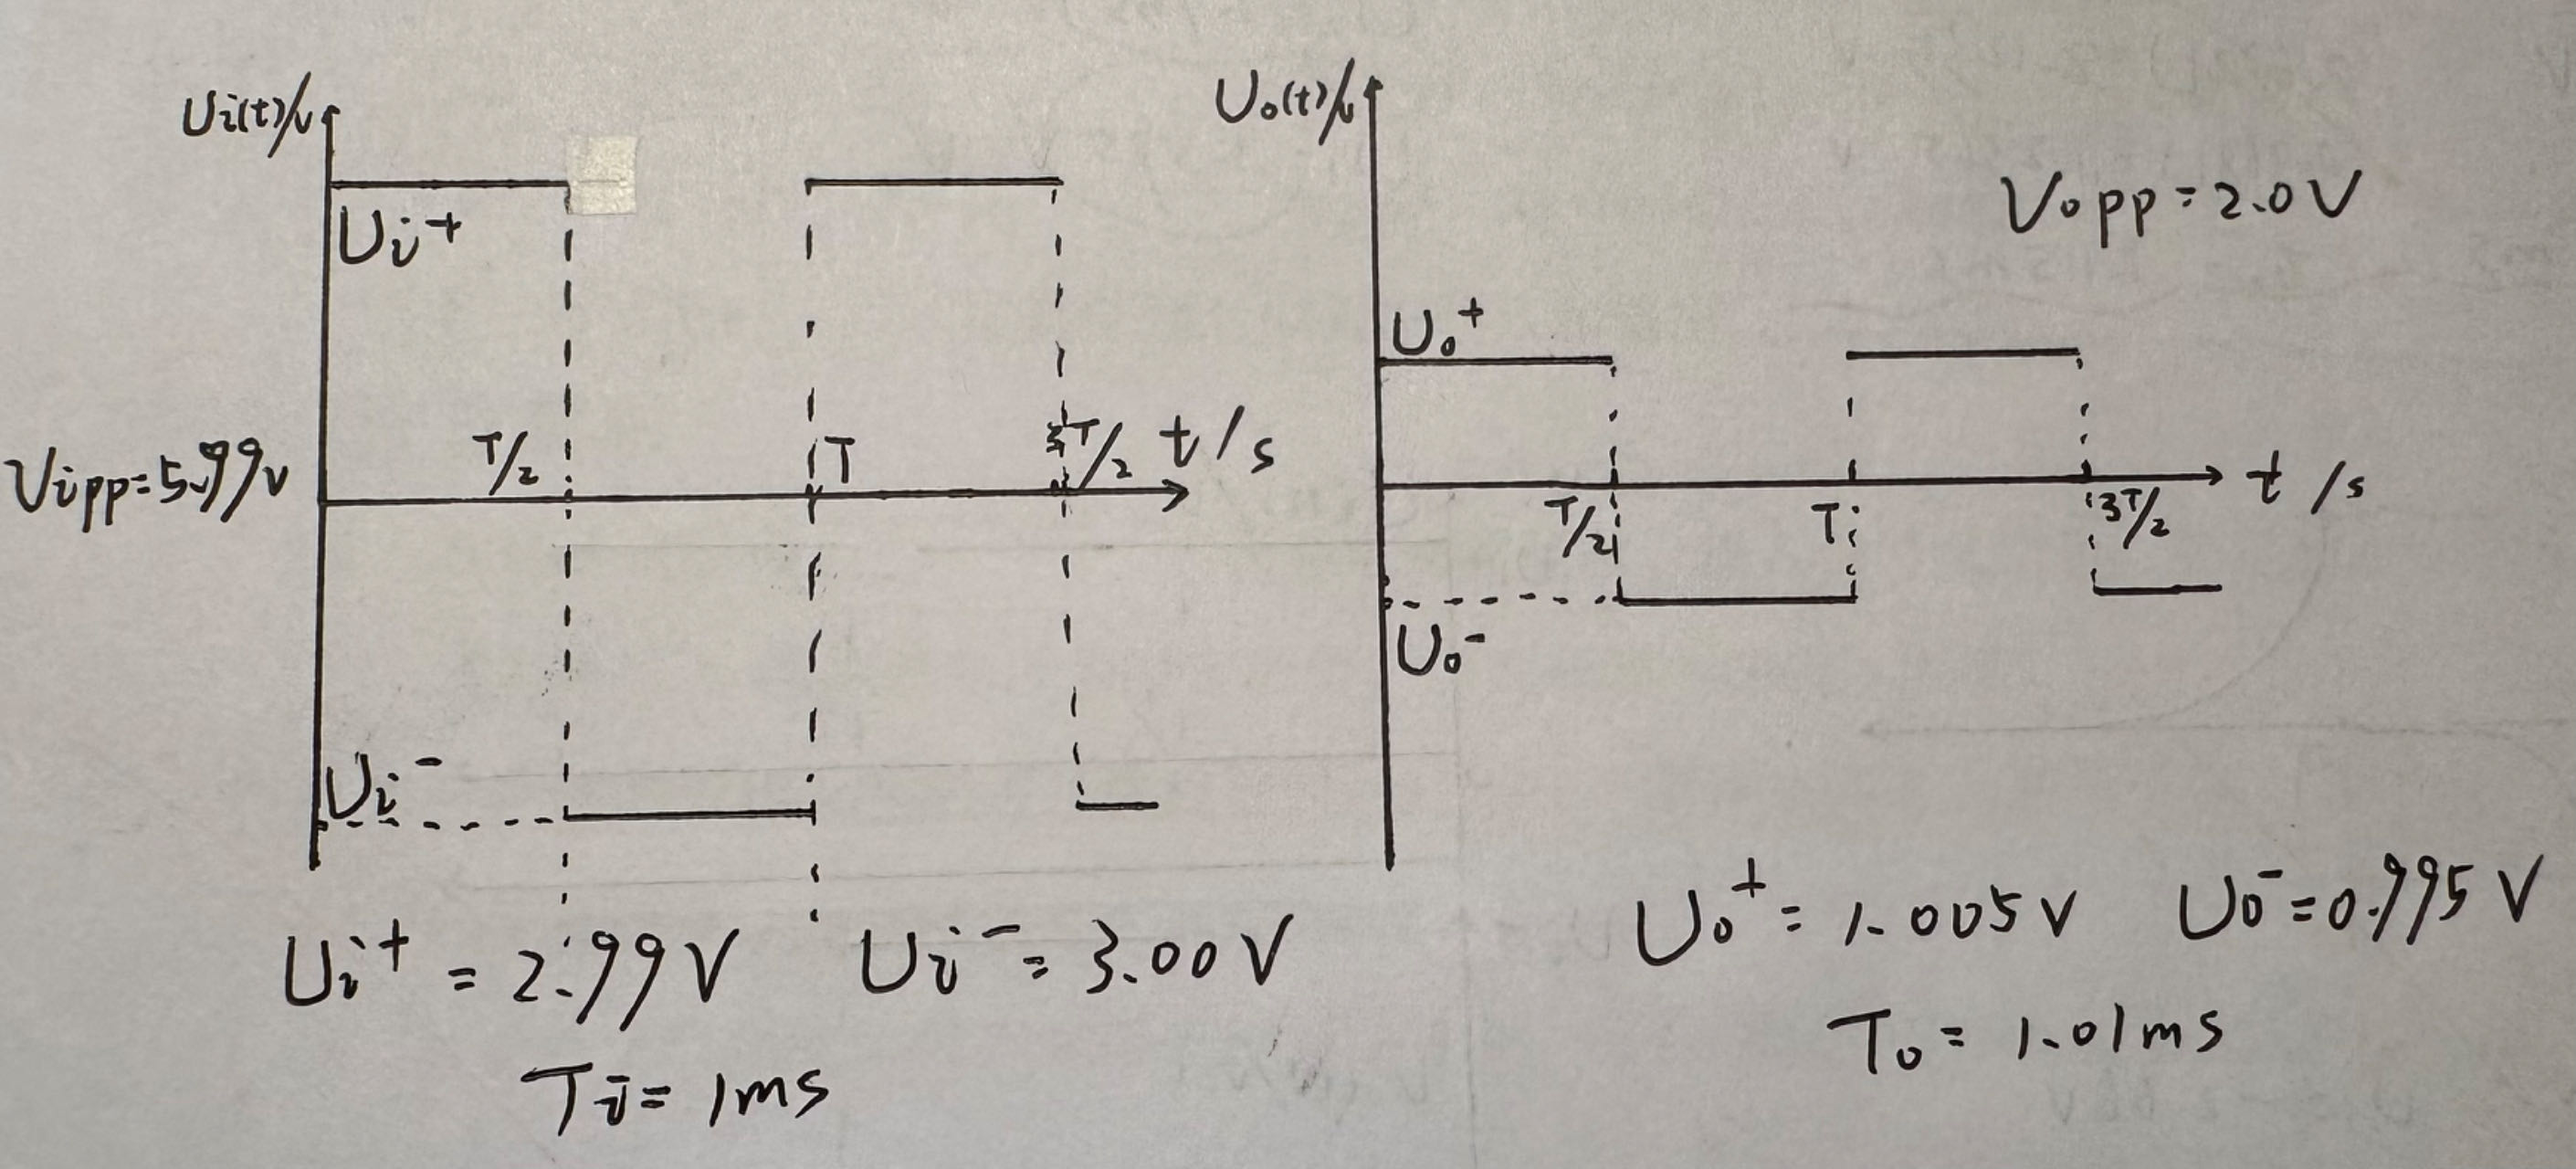
\includegraphics[scale=0.1]{16}}
        \centering
        \caption{\small 图十二:实验四相关图片}
    \end{figure*}

    \vspace{1cm}


    \section{注意事项}\label{sec:6}
    \noindent
    {1.在做零状态和零输入、积分、微分电路实验时,输入信号选定为方波输出,输出幅度是电阻$R_{1}$两端电压归定的值,即为所要求的输入电压。}

    \noindent
    {2.从示波器上记录被测信号的波形时,时域时一定要先确定X轴的位置,即零电平的位置,垂直方向耦合方式选择为$DC$。}

    \vspace{1cm}


    \section{思考题}\label{sec:7}

    \subsection{在实验电路图3-8中,电阻$R_{1}$在电路中起什么作用?}\label{subsec:q1}
    \noindent
    {答:1.$R_{1}$的接入是为了在二极管截止时给 RC 串联电路提供一个闭合回路,使电容上的电压放电 时存在一个回路,这样才能观察到电路的零输入响应。}

    {2.$R_{1}$有传递电压的作用,通过测量$R1$两端的电压,可以得到输出电压。在本实验中输出电压为5V。}

    \subsection{本次实验中,能用毫伏表测量电阻$R_{1}$两端的矩形波电压吗,为什么?}\label{subsec:q2}
    \noindent
    {答:本次试验中不能用毫伏表测电压。毫伏表是按照正弦电压有效值测量电压的,如果被测信号并不属于正弦电压,则无法测定准确,比如采用方波电压等等。若要使用毫伏表测量,需要经过复杂的整流过程。因此,本次试验中不可以用毫伏表测量电压,而应该使用双踪示波器。}

    \subsection{根据本次实验说明$RC$电路分别作为微分电路和积分电路,必须具备的条件?}\label{subsec:q3}
    \noindent
    {答:1.积分电路:输出信号与输入信号的时间积分成正比的电路。应具备的条件是:$RC \ge T_{k}$,其中$T_{k}$是脉冲周期, 积分电路可将矩形脉冲波转换为锯齿波或三角波,还可将锯齿波转换为抛物波。 电路的时间常数必须要大于或等于10倍于输入波形的宽度。}

    {2.微分电路:输出电压与输入电压的变化率成正比的电路。 应具备的条件是:$RC \le T/10$,其中$T$是输入信号的周期, 微分电路可把矩形波转换为尖脉冲波,电路的时间常数必须要小于或等于1/10倍的输入波形的宽度。}

    \vspace{1cm}


    \section{实验总结}
    {此次实验完成了对一阶电路零输入相应、零输出相应、全响应过程、微分电路、积分电路和脉冲分压电路的波形的观察,测量了电路重要的参数时间常数,同时掌握了形成微分电路、积分电路的条件,达到了实验要求,完成了实验目的。}\label{sec:8}

%    \bibliography{main}
%    \bibliographystyle{plain}

\end{document}
